\documentclass[11pt,a4paper]{report}
\usepackage[utf8]{inputenc}
\usepackage[english]{babel}
\usepackage{amsmath, amssymb}
\usepackage{csquotes}
\usepackage[acronym]{glossaries}
\usepackage{graphicx}
\usepackage{xcolor}
\usepackage{tikz}
\usepackage{eso-pic}
\usepackage{listings}
\usepackage{tabularx}
\usepackage{times}
\usepackage{setspace}
\usepackage{float}
\usepackage[a4paper,top=18mm,bottom=26mm,left=30mm,right=30mm,headheight=14pt,footskip=14mm]{geometry}
\usepackage{titlesec}
\usepackage{hyperref}  
\usepackage{xurl}
\Urlmuskip=0mu plus 1mu
            \hypersetup{backref=true,       
                    pagebackref=true,               
                    hyperindex=true,                
                    colorlinks=true,                
                    breaklinks=true,             
                    linkcolor=black,  %idk
                    urlcolor=blue,    %href
                    filecolor=blue,   %table of content
                    citecolor=red     %citations
}

\usepackage{attachfile2}

\usepackage{hyperref}
\usepackage{cleveref}


\usepackage[backend=biber,style=numeric,sorting=none]{biblatex}
\addbibresource{ref.bib}
\ExecuteBibliographyOptions{doi=true,url=true,eprint=true}
\AtBeginBibliography{%
    \sloppy
    \setlength{\emergencystretch}{3em}
}


% ----------------------------------------------------------- %
% TODO: Check pdf's title
\hypersetup{
    pdftitle={Master thesis - Louis Devroye - 2025-26},
    pdfauthor={Louis Devroye (Louis.Devroye@ulb.be)},
    pdfsubject={Fault-Tolerant Microarchitectures: Fault recovery by rewinding enclaves in a Trusted Execution Environment on a RISC-V architecture (Keystone)},
    pdfkeywords={Microprocessor, Fault-Tolerant, Fault, Redundancy, Cybersecurity, Microarchitectures, Keystone, Checkpointing, Rewind, Enclaves, TEE, RISC-V, open-source},
}

\newcommand{\thisyear}{\the\year}
\newcounter{oldyear}
\newcommand{\lastyear}{\theoldyear}
% useless as \chapter starts a new page
%\newcommand{\newchapter}{\newpage\chapter}

\newcommand{\subtitle}[1]{%
    \posttitle{%
    \par\end{center}
    \begin{center}\large#1\end{center}
    \vskip0.5em}%
}


\newcommand\addbackground{%
  \AddToShipoutPictureBG*{%
    \begin{tikzpicture}[remember picture,overlay]
        \node[anchor=center] at (current page.center) {   % change north w/ center, etc.
            
\includegraphics[width=0.45\paperwidth]{sceau.png}%
        };
    \end{tikzpicture}
  }%
}

\newcommand\clearbackground{%
  \ClearShipoutPictureBG%
}

\titlespacing*{\chapter}{0pt}{-1.2em}{0.8em}
\titlespacing*{\section}{0pt}{0.5em}{0.3em}
\titlespacing*{\subsection}{0pt}{0.4em}{0.2em}

%COUNTER-------------------------------------------------------  %%%
\newcounter{todocounter}

\newcommand{\TODO}[1]{
    \stepcounter{todocounter}
    \textcolor{red}{\\\textbf{TODO \thetodocounter:}}
    \MakeUppercase{\textbf{#1}}\\}

\newcommand{\stepandprint}[1]{%
  \csname the#1\endcsname%
  \stepcounter{#1}%
}

\newcommand{\resetcounter}[1]{
    \setcounter{#1}{0}
}

% Clickable source link that also embeds the file inside the PDF.
\newcommand{\srcattach}[2]{%
    \textattachfile[icon=Paperclip,color=0 0 0]{#1}{\texttt{#2}}\\
}

\newcommand{\github}{%
    \href{https://github.com/ldevroye/keystone/tree/master}{GitHub repository}
}

\newcommand{\keystonegithub}{%
    \href{https://github.com/keystone-enclave/keystone}{Keystone repository} \cite{keystone-repo}
}



%-------------------------------------------------------%
\begin{document}
\onehalfspacing

\setcounter{oldyear}{\year}
\addtocounter{oldyear}{-1}
\setlength{\textwidth}{145mm}

\begin{titlepage}
\begin{center}
\begin{minipage}{\textwidth}
\begin{Large}
Faculty of Sciences
\hfill
Departement of Computer Sciences
\end{Large}
\end{minipage}
\\[1cm]

\includegraphics[scale=0.15]{img/sceau.jpg}\\[1cm]

\begin{minipage}{\textwidth}
\textsc{Master thesis}
\end{minipage}\\[0.5cm]

% Title
\rule{\textwidth}{1mm}
\centering
\textbf{\huge Fault-Tolerant Microarchitectures: Enhancing Reliability through Redundant Execution\\[0.2cm] }
\rule{\textwidth}{1mm} 
\vspace*{1mm}

\LARGE \textbf{Author :} DEVROYE Louis\\[0.2cm]
\LARGE \textbf{Advisor :} MÜHLBERG Jan Tobias\\[0.2cm]
\LARGE \textbf{Director :} MÜHLBERG Jan Tobias\\[0.2cm]

\vfill
% Bottom of the page
\Large Academic year \lastyear--\thisyear
\end{center}
\end{titlepage}






%%%%%%%%%%%%%%%%%%%%%%%% ABSTRACT
\begin{abstract}
\TODO{ABSTRACT at the end}
\end{abstract}


% \chapter{Acknoledgments}

\tableofcontents


%%%%%%%%%%%%%%%%%%%%%%%% INTRODUCTION %%%%%%%%%%%%%%%%%%%%%%%%
\chapter{Introduction}

% INTRO
Microprocessors are getting more efficient each year due to miniaturization of transistors \cite{silicon}. 
However, this rise in efficiency comes with the pricey cost that are faults. 
Critical systems are particularly vulnerable considering the stakes (human lives) and the real time constraints such as time, temperature, computational power or even voltage. 
This field is not new \cite{vonneumann56, n-version85} but is still drawing attention, has a lot of gaps yet to be covered and is structuring, mostly around the type of faults and the way to deal with them \cite{future-research}.
\\

%FAULT DETECTION & CORRECTION
Fault detection is a wildly studied field \cite{fault-detection-survey}, it is a pillar for critical systems and for networks. 
The detection goes along with Error Correction Codes (ECC), these are mostly used in network due to the necessity to get the good informations using as little of time/computation as possible. 
However, these techniques come with a lot of overhead and assumptions that cannot be made in this field. 
First, network consider the source to be viable, when a request is made to a server, the informations are checked, let's say with a basic checksum. 
In micro architectures, the sensors would be the parallel to the server. 
However, the data given by the sensor are not known to be true or false (exception made for specific cases, for example if a distance check returns a negative answer). 
Secondly, all the layers needed to prevent a fault from happening, in TCP for example, would be too costly to just put in a micro processor, in overhead (from both computation and memory standpoint) and in time needed. 
In fact, the main topic is that these systems are time bounded, so it is important to be able to have the, correct, data before a certain deadline. 
Unfortunately, all theses constraints do not apply, at least not all at once, to networks.
\\


% SW time based
On the other hand, a lot of programs and studies are focused on \textit{Software Implemented Fault Tolerance} (SIFT) and more precisely on \textit{time redundancy} methods, they are solely interested in making fault-tolerant programs that meet deadlines. 
That is in itself an honorable (and complex) goal, yet one of the main problem, related to this topic, with miniaturization being the increase in temperature. 
One could argue that making extra computation or overclock the CPU when an error occurs, possibly because of the aforementioned heat, wouldn't make any sens. 
In fact, it could slow the whole system (to cool down) or cause more fault at the time being and it would strain the system even more on the long run \cite{other-goal,bachelor-thesis}.
\\


% ALTERNATIVES TO TIME 
To improve this contradictory aspect, some research has been done. 
They put the light on other aspects than only timing constraints (while keeping the reliability). 
For example, power and energy consumption as the \textit{Internet of Things} (IoT) develops \cite{iot} is gaining more attention.
\\

% HW also
Hardware is the basis off all this domain and because of this, extensive work can be done directly on it to prevent or recover from faults directly on the hardware. 
This approach deletes most of the overhead of the software techniques but it is much more restricted and complex than implementing and debugging a layer over a "simple" hardware structure. 
\\

% CYBERSEC
Moreover, this subject can be extended to \textit{cybersecurity} in a way to harden the task (or at least the conception) of malicious programs \cite{diversification-obfuscation}. 
In fact, an attacker could try to reverse engineer a program, he could also try to check the memory for data or the CPU usage and instructions or even using the power supply as an attack vector \cite{ARM-TrustZone-CortexM} to prevent a task from completing. 
For this purpose, several techniques have been developed to try and block either the static or dynamic analysis of a program \cite{diversification-obfuscation}. 
Even measuring the redundancy of a program to be able to scale and compare two diversification technique and choose one for example \cite{measure-redundancy}. 
The research could even separate the low-level redundancy from a high-level, algorithmic, one.
\\

The research question of this thesis is whether rewind on RISC-V processors for opaque enclaves in an unsecure world makes sense.
It is interesting because the baseline answer is yes, but the cost it implies and the security it requires make the answer less obvious.
This thesis studies rewind and discard, the hardware support around PMP and Keystone, the cycle overhead, and the cybersecurity properties that decide whether the mechanism is acceptable.
It also looks at the conditions under which rewind remains useful and the conditions under which it becomes too expensive or too fragile.
The reader should read this thesis to understand the practical limits of rewind, the assumptions it depends on, and the trade-off between recovery and overhead.
\\


Furthermore, the codebase (implementation of the checkpoint and rewind enclave, host and tests) of this thesis can be found on the \github. 
This is a fork of the main Keystone github \keystonegithub. 
The files can also be found in the Appendix (\ref{chap:appendix}).




%%%%%%%%%%%%%%%%%%%%%%%% SotA %%%%%%%%%%%%%%%%%%%%%%%%
\chapter{State of the Art}
\label{chap:SotA}

% INTEREST
\section{Engagment in the scientific community}
For as long as computers (some could even say tools in general) have existed, so have defaults, errors and bugs \cite{vonneumann56}. 
However, the need for a solid structure and concretes answers increased as Moore's law kept going on \cite{moore-law}. 
This topic is drawing more attention as the years go by.

% FAULTS
\section{Faults}
Faults are the basis of the problem but the outcome a of fault, and they way it is handeled, is equally important. 
To be clear and rigorous, we will use the Institute of Electrical and Electronics Engineers' (IEEE) \cite{future-research, ieee, other-goal} standards.
In this goal, we can separate a fault and its consequences in 3 categories each one following from the previous one:
\begin{itemize}
    \item \textbf{Fault}: A defect in a hardware device or component. 
    It can be a \textit{Single Event Upset} (SEU), otherwise seen as a bit flip or it can be other models such as \textit{Multiple Event Upset} (MEU).
    \item \textbf{Error}: The difference between a computed, observed or measured value or condition and the true, specified, or theoretically correct value or condition. 
    It is the effect of a fault on the system.
    \item \textbf{Failure}: The inability of a system or component to perform its required functions within specified performance requirements. 
    In other words, the program malfunction due to an error.
\end{itemize}

Now, we need to categorize faults \cite{future-research, other-goal}
\begin{itemize}
    \item \textbf{Transient}: Produces a temporary effect on the system in a very short period of time. 
    It is often modeled using SEU. They are most likely cause by :
    - \begin{itemize}
        \item alpha radiation (due to cosmic radiation or nuclear fission)
        \item electromagnetic interference
    \end{itemize}
    \item \textbf{Intermittent}: Livespan similar to \textit{Transient} but it occurs in \textit{burst}. 
    It is mainly caused by eternal conditions : temperature, voltage, hardware wear out and High Intensity Radiated-Field (HIRF)   
    \item \textbf{Permanent}: Results from hardware wear out or manufacturing defects. 
    The only fix for this type is to repair or change the hardware. 
    Component wear out is well known in the current literature, the \textit{Bathtub curve} \cite{bathtub} describe the three main phases of a component's life : 
    \begin{itemize}
        \item The \textit{infant} stage is when the hardware is fairly new (not in term of design). 
        Thus, it might be defective while still passing the basic tests required for using it. 
        As this phase goes on, the average error rate decreases.
        \item The \textit{main} stage is, for the main part, the longest one. 
        The component is viable (since it has passed the previous phase) and not yet worn out. 
        But still random faults occurs (due to environment, etc.). This phase is the best in term of fault rate (which is supposedly constant).
        \item The \textit{wear out} stage is the first that comes to mind when speaking of permanent faults. 
        A part of the component is defective and there is no direct fix except for replacing/repairing this part. 
        In opposition to the $1^{st}$ phase, the average error rate increases over time.  
    \end{itemize}

    %% IMG bath curve
    \begin{figure}[H]
        \centering
        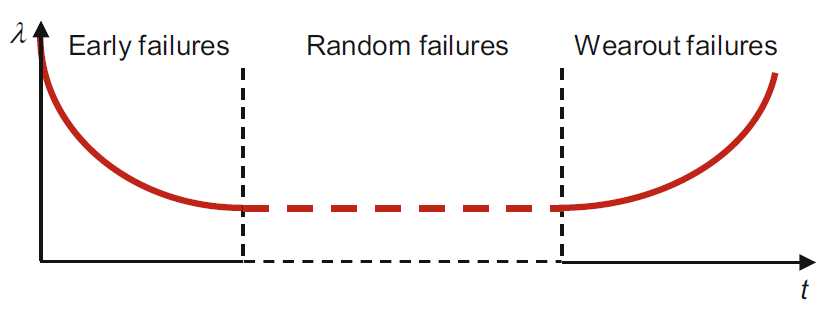
\includegraphics[width=0.8\linewidth]{img/bathtub.png}
        \caption{Bathtub curve. "Typical plot of the $\lambda$ failure rate over time $t$ (bathtub curve) with decreasing, constant, and increasing failure rate sections" - Fig4.4 (p52) \cite{fundamentals}}
        \label{fig:bathtub}
    \end{figure}
\end{itemize}


\section{Fault Recovery Techniques}
\subsection{Space Redundancy}
\begin{itemize}
    \item \textbf{N-modular redundancy (NMR)}: this consists of $N$ (2,3,4,..) instances of the job $i$ running at the same time, when the job $i$ finishes, a vote start and the majority is returned as the result. 
    NMR can detect by essence and correct the error. 
    However, it is important to note that it can only detect an \textit{error}, not a \textit{fault} \cite{future-research}. 
    Also, each $n$ instance of the job $i$ should run on different cores to avoid SEU. 
    
    \item \textbf{standby redundancy}:
    \begin{itemize}
        \item \textit{Hot} standby is when the backup system runs in parallel with the main one. 
        If something fails, the switch to the backup is almost instant since it is already active and synchronized.
        \item \textit{Cold} standby is when the backup system is off until the main one fails. 
        When that happens, the backup starts up and takes over. 
        This takes longer but saves resources while things are working.
    \end{itemize}
\end{itemize}
\subsection{Time Redundancy}

\begin{itemize}
    \item \textbf{re-execution}: This technique runs the same task again to see if the error happens in the same way. 
    If the second run works fine, the first one probably had a temporary problem. 
    It helps filter out transient faults. It has two main approaches:
    \begin{itemize}
        \item \textit{Backward error recovery}: If the state of the job or the environment needs to be restored after a fault, then the faulty job is restarted.
        \item \textit{Multiple recovery}: due to scheduling reasons, the currently preempted jobs are also re-executed even if not affected by the fault. 
    \end{itemize}
    
    \item \textbf{Checkpoint}: A checkpoint saves the state of the system at a certain time. 
    If a failure happens later, the system can roll back to this saved state and continue from there without starting over from scratch. 
    It is often used in High Performance Computing (HPC) for long running tasks and in the industry in general as it is effective.
    
    \item \textbf{Recovery blocks}: This method runs a primary version of a task and checks the result. 
    If the result fails, it runs another version (possibly degraded) to try again. 
    This can repeat with more versions if needed until one gives a good output.
    
    \item \textbf{Forward error recovery}: Mostly used in networks, it executes a special routine that fixes the error without re-executing the original task. 
    Simple raise/throw exception handling. 
\end{itemize}


%%% IMG main 4
\begin{figure}[H]
    \centering
    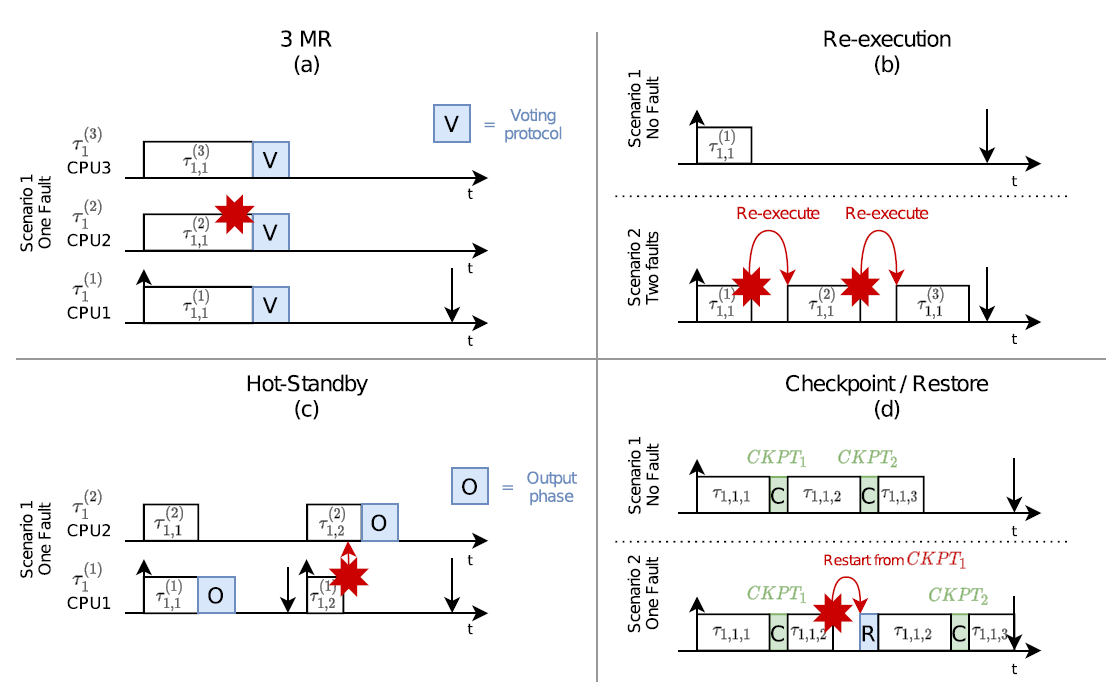
\includegraphics[width=1\linewidth]{img/main_recovery_techniques.png}
    \caption{The four main fault recovery approaches. \\"In (a), (b), and (c), the symbol $\mathcal{T}^{(k)}_{i, j}$ represents the $j^{th}$ job of the $i^{th}$ task, and $k$ identifies the redundancy or re-execution job. Instead, in (d), $\mathcal{T}_{i,j,k}$ is the $k^{th}$ part of the job $\mathcal{T}_{i, j}$ . In the depicted example, the job $\mathcal{T}_{1,1}$ is composed of three parts" - Figure 1 of \cite{future-research}}
    \label{fig:main_recovery_techniques}
\end{figure}


\subsection{Fault Detection}
Even though it is not the main topic, neglecting fault detection would be just as bad as neglecting any part of the domain. 
To highlight this, we can note that \textit{NMR} does recover from an error occurring but it can \textit{not} detect the underlying fault. 
Preventing the faults as soon as possible save the whole recovery process and thus saving the additional computational power, possibly missed deadlines (in mixed critical systems for example) or even heat-induced wear out. 
\subsubsection{Hardware}
\begin{itemize}
    \item \textbf{Fail-signal processor} is used in multi-processor architectures. 
    A processor complete the task and another one checks for abnormalities (time or result) on the first one.
    \item \textbf{Error detecting code} (EDC) are used to detects errors (for example checksum). 
    It is used in the memory, the bus and on networks.
    \item \textbf{Error correcting code} (ECC) are used along EDC to try and correct small errors. 
    They often need a matrix to be able to find the errors confidently. 
    \item \textbf{Watchdogs}is used for the timing constraint. It ensure that is is respect.
\end{itemize}
\subsubsection{Software}

Hardware has the benefit of not affecting execution time because it works in true parallel. 
It can run checks or backups at the same time as the main task without slowing things down.
For software, we have to consider the worst-case execution time of tasks along with the extra time used by the checks added to each job. 
Software can use multithreading to help, but the extra cost is still there.


\subsection{Fault Injection}
Designing and implementing a system without tests cases is not imaginable. 
To this end, fault injection is being used. The idea is quite simple, put the system under various stress tests to check its tolerance to faults. 
This allows the use of a critical micro processor with no more reluctance than necessary. 
These injections are made using four different techniques. \cite{diversification-obfuscation, future-research}
\begin{itemize}
    \item \textbf{Hardware}-based: Connect a device to mess with the system, for example with voltage spikes or imputing RF disturbances. A simple approach, yet effective. 
    \item \textbf{Software}-based: Use a program to mess with the memory allocation of the system, for example allocating random or predefined segments. It is also also fairly simple. 
    \item \textbf{Simulation}-based: The hardware is \textit{simulated} and faults are injected through registers using pseudo-random/predefined patterns. This gets more complicated.
    \item \textbf{Emulation}-based: The hardware is fully \textit{emulated} by being written on a Field-Programmable Gate Array (FPGA). This allows host to inject faults in a transparent way (like a real fault would occur). 
\end{itemize}


%------------------------------------------------------------------%
% CRITICALITY
\section{System's criticality}
Critical systems are nearly everywhere today, from aviation \cite{avion-fault-timing-multi} (DAL) to hospitals. 
A lot of the critical embedded systems are in the Internet of Things (IoT). 
To address such variety, we can use the Mixed-Citical models. 
These models consist on prioritizing the tasks with higher importance. 
For example, a task that needs to check if the distance with the car in front of you is large enough if more important than the one that checks the temperature. 
If the former fails, a crash might happens as if the latter fails, temperature might go up by 0.1°C. 
The formal way of doing this is to map a number (the priority) to tasks, 0 being the most critical ones and as the number increases, the priority lowers. \\

The most common, to our knowledge, mixed critical model is the \textit{Dual} \cite{scheduling-mixed}. 
It consists of two priority :
\begin{itemize}
    \item HI-critical
    \item LO-critical
\end{itemize} 
As the names suggest, the HI-criticality stands for tasks that need to be finished in time (with a high priority) and LO-critical is used to describe tasks that can be dropped or can miss a deadline (low priority).
The software failure model of a task is usually considered in two senses: \begin{itemize}
    \item the logical sense: the task produces an incorrect output
    \item in the timing sense: the task does not produce a correct output by the end of its deadline
\end{itemize}
However, all the industries (aviation, automobile, medicals, railway, spaces, industrials, etc.) have their own priority scale. All of them are, to some extent, a specification of a simple Mixed critical system with task priorities. 
For example, aviation with \textit{DO-178B} (or C) with the DAL priority that goes from A to E, A being the most critical and E being the least. 


%---------------------------------------------------------------%
% CYBER
\section{Cybersecurity}
Cybersecurity is also a main point of attention in this field (as it is a field itself). 
This is even more valid with the growth of the IoT in general on this past decades and this growth increased with the new arrival of Artificial Intelligence (AI) \cite{iot}.
This section will cover the basics of this project that we will use.

\subsection{Threat Model}
A threat model is a structured description of what must be protected, who may attack it, and which assumptions are accepted by the system.
It helps separate the trusted part of the design from the untrusted environment and makes the security claims explicit.
It is useful because the analysis depends on the untrusted parts, the trusted ones, the storage channel and the recovery path not having the same level of trust.
It also makes clear which attacks are in scope, which assets must remain confidential or intact, and which limitations are acceptable for the chosen platform.
\\

In this work, the threat model is especially important because the enclave must recover in an untrusted world while still preserving the checkpoint contents and the control flow of the recovery mechanism.
This provides the basis for the later discussion of TEEs, enclaves, and the rewind protocol.
\\

% TEE
\subsection{Trusted Execution Environments (TEE)}
A Trusted Execution Environment (TEE) \cite{TEE} is a secure part of the processor that runs code and handles data in isolation from the rest of the system. The goal is to protect sensitive operations from malware, faulty software, or even privileged system components like the OS or hypervisor. TEEs are often used for secure key storage, encryption, authentication, and digital rights management. 
It contains enclaves and is often run on \textit{ARM TrustZone} for mobile devices \cite{ARM-TrustZone-CortexM}.

% ENCLAVEs
\subsection{Enclave}
Enclaves provide isolated execution environments that protect sensitive code and data even if the Operating System (OS) is compromised \cite{enclave}. 
They rely on hardware-level support (TEE) to keep the enclave memory hidden from other software, reducing the attack surface. Enclaves help contain faults, data and prevent them from spreading beyond their boundary, adding both security and resilience. It is used on mobile for example to provide a safe environment for banking, cryptographic or even biometric data storage. 
This is to avoid any third party software being able to access confidential data.

% Code obfuscation & diversification
\subsection{Code obfuscation \& diversification}
Code obfuscation and diversification make it harder for attackers to understand or predict the system’s behavior. Obfuscation transforms the code into a version that works the same but is harder to analyze (static analysis). Diversification changes the memory layout, instruction set, or data locations across runs or devices. 
These techniques slow down attacks and can stop malware that depends on known patterns, making the system more fault-tolerant against targeted exploits (Zero-day vulnerability for example).

%REWINDING \& DOMAINS
\subsection{Rewinding \& Domains}
A current approach to address attacks is to first detect the attack and then roll-back the system to a previous (supposedly) safe state by replications or checkpointing. As much as this mechanism works to ensure reliability of the system, the \textit{resilience} and \textit{availability} when it is under an attack is not the focus. This last point enables an attacker to use the delay of roll-backing the system as an attack vector. To solve this, a software library has been created for 64-bits x86 processors : \textit{Secure Domain Rewind and Discard (SDRaD)} \cite{sdrad}. The underlying logic consists of using \textit{Domains}, compartmentalized and secured spaces and using a domain for each critical task. Thus, when an error occurs, the corrupted domain can be \textit{discarded} (terminated) and the error can be handled. In this scenario, the targets services are Commercials Off-The-Shelf (COTS) processors \cite{sdrad, fault-detection-survey, future-research} (ie. processors that don't need hardware specifications or specific changes in order to work) for web services with multiple clients. The plurality of the clients is where the danger lies as if one client is malicious, it can affect the others. 
That is where the SDRaD mechanism comes in place, each client or subroutines of the clients could be stored in different domains making a great isolation in-between clients. 
The program using the library can rewind the states of the domains discarded to avoid propagation and this makes the possible Denial of Service (DoS) attack outdated as the states are saved frequently and the whole system does not need to restart from scratch (using caches services for example). 


% DATA & CONTROL FLOW
\subsection{Data \& Control flow}
Protecting data flow and control flow is key to stopping many types of (dynamic) attacks. Data flow checks make sure sensitive data does not leak or get overwritten. 
Control flow is the instructions order of execution for the CPU. 
Hardware or software guards can stop faults caused by memory corruption, buffer overflows, or instruction hijacking. 
Together, these methods help prevent faults from becoming full system breaches.

% measurement
\subsection{Obfuscation measurement}
A derivation of this is the layout obfuscation, it consists only on destructuring the program. 
This is mainly done to prevent a human reading the code base and reverse engineer the whole system (thus gaining informations and understanding of possible breaches). 
This a a one way approach as when the structure is deleted (when classes are merged for example or comments and name deleted) it cannot be found afterwards. 
\textit{Potency} and \textit{Resiliency} are used to measure this \cite{measure-redundancy}, the former is to measure human readability and the latter is used to measure how well the system resists to automated decompilers/deobfuscators/deassemblers \cite{diversification-obfuscation}. 


% LIMITATIONS
\subsection{Limitations}
One of the goals is to make the system more resilient to attacks and thus to rise the cost of developing attacks that could harm the system \cite{diversification-obfuscation} (this is seen as control flow). 
Another one is to prevent someone with malicious intent to comprehend the system (static analysis) or even if they do, to prevent them understand the flow of the program as it runs (dynamic analysis).
However, as for every domain (in computer science), there are limitations. 
These inherent limitations are that no system is full proof. 


\subsection{Background work}
\TODO{related work that's already done, that we're basing ourselves of.}
% papers
\cite{sdrad,ARM-TrustZone-CortexM}






%%%%%%%%%%%%%%%%%%%%%%%% PROBLEM %%%%%%%%%%%%%%%%%%%%%%%%
\chapter{Problem Statement and Objectives}
%% theoretical assumptions
Now that everything is, roughly speaking, well defined. 
Although the whole domain is very interesting and always needs specific studies on various topics, it needs to be narrowed down in order to suit a Master thesis.

First cut is the type of \textit{redundancy}. 
For the purpose of the research, the tests will be based on the \textit{timed} redundancy method that is \textit{rewinding} agains't no redundancy. 
This allows to measure the viability and the relevance of the work done. 

Second cut is the type of systems that needs to be modeled. 
Our focus will be \textit{one level} criticality system, as they are great will reflect an encalve that has one single job.
There could be extended work on several enclave levels that have a different saving rates. Making it mixed criticals enclaves of a bigger system.

Third cut is the type of faults. 
As diving in any type of fault could be a thesis in itself, the faults will be reviewed only for what they are and not necessarily for their cause. 
Thus, \textit{all three types} will be looked upon.

Next cut is the channel that will be use. 
In other terms, \textit{hardware} and \textit{software}. 
As they are both important and linked in various ways. 
The focus will not only, at least initially, be on one of them but rather on \textit{both} using \textit{emulation} and the implication that each have on the other. 
For example, Enclaves that need restricted access and create a waterfall of complexity in the design and implementation has on impact on both hardware and software. 
To the extent, we will base our work on \textit{Keystone} that provides a platform to emulate a RISC-V processor with enclaves and cryptographic soundness using hardware (PMP) on a TEE. 
(\cite{keystone-repo, keystone-web, keystone-docs}), This will be detailed in the corresponding Chapter \ref{chap:Keystone}.

Final cut is about the \textit{cybersecurity} perspective. 
As the industry around this domain is mostly critical (aviation, automobile, space or even medical), there is a high risk with someone getting access to something they shouldn't have. Considering that, we must ensure that the faults occurring, possibly from a malicious source, does \textit{not break the system nor give informations} about it. 
Not much from a static analysis (reverse engineer) perspective but rather from a \textit{control flow} one. 
To make it more precise, on TEEs when a fault occurs, the system can try to change of enclave as if it was a \textit{Domain}. 
Then the system can be rewinded and set to a safe state while not being unavailable.
\\

These specifications can be linked to try an extend the SDRaD \cite{sdrad} work in a TEE, making an equivalence between domains and enclaves. 
As the enclaves are subregions of a TEE, they are isolated and secure as the definition of a domain using Private Keys for Userspace (PKU) and Memory Protection Keys (MPK) (with register mechanism and much more \cite{sdrad}). \\

Therefore, the research should focus on \textit{Fault recovery by rewinding enclaves in a TEE on a RISC-V architecture using Keystone} and extending existing works.
The main objective is to determine whether rewind is practical for opaque enclaves on Keystone when the world outside the enclave cannot be trusted.
The first sub-objective is to measure the cost of checkpointing, loading, and ordinary execution so the break-even point can be identified.
The second sub-objective is to verify that the recovery path still satisfies confidentiality, integrity and authenticity, atomicity, and unclonability.
The third sub-objective is to connect these measurements to the system design choices in PMP, enclave isolation, and the sealing protocol.
Together, these objectives answer whether rewind is useful in practice and what the implementation must assume to make it safe.
\\








%%%%%%%%%%%%%%%%%%%%%%%% Keystone Structure %%%%%%%%%%%%%%%%%%%%%%%%
\chapter{Keystone Structure}
\label{chap:Keystone}
"Keystone is an open framework for architecting trusted execution environments (TEEs) based on hardware enclaves. Keystone aims to provide an easy way of architecting and building a customized TEE for an arbitrary RISC-V platform with a simple workflow. 
This allows the TEE to be highly optimized for better performance, smaller trusted computing base (TCB), and programmability with a given workload and a threat model." 
- 2.2. Keystone Basics \cite{keystone-docs}
\\\\
Its implementation can be found on the corresponding github reposity: \keystonegithub.
\\
The corresponding documentation can be found at :
\href{https://docs.keystone-enclave.org/en/latest/index.html}{https://docs.keystone-enclave.org/} 
\cite{keystone-web,keystone-docs}


\section{RISC-V}
RISC-V is a free and open-source (in contrast to x86 and ARM) Instruction Set Artchitecture (ISA).
Due to its reduced instruction set, it has become a popular architecture for embedded systems and microcontrollers as it allows to reduce power consumption, code size, and memory use. \cite{riscv-manual}
\\

RISC-V has three priviliege levels (2.1.2. RISC-V background \cite{keystone-docs, review-keystone}):
\begin{itemize}
    \item U-mode: User processes
    \item S-mode: Kernel
    \item M-mode: Bootloader-firmware
\end{itemize}

M-mode is the highest as it controls physical ressources and interrupts. 
It is analogous to microcode in Complex Instruction Set Computer (CISC) ISAs (x86).
However, unlike microcode, it is implemented in existing programming languages (C) and toolchains (gcc).
This makes it much more accessible.  
\\

The running software can thus not being interfered or interuppted by lower modes.
In Keystone, the M-mode is used for:
\begin{itemize}
    \item the Security Monitor (SM)
    \item the Trusted Computing Base (TCB)
\end{itemize}
As all of these are software implementation. It is much easier to implement, debug and fix than it would be on hardware.

\subsection{Physical Memory Protection (PMP)}
\label{sub:pmp}
"Physical Memory Protection (PMP) is a part of the RISC-V Privileged Architecture Specification which discribes the interface for a standard RISC-V memory protection unit." 
- \cite{SiFive}
It alows the M-Mode to control physical memory access.
PMP is ruled by a set of Control Status Registers (CSR) to restrict physical memory access for U and S mode and is configured by the M-mode.
\\

PMP as a variable number of entries depending on the the platform it is on. 
The one in our interest is QEMU, its virtual machine have 16 entries, each entry is defined by one or more CSRs.
It works on physical addresses, the configuration of the subsequents virtual adresses can be let to the S-mode without compromising security.
Even with different hardware implementation, the standard garantees basic functionality. 
\\

More importantly, PMP is used by the SM to create memory isolation and can be dynamically configured by the M-mode (using CSRs).

\subsection{Security Monitor (SM)}
\label{sub:sm}
Is the root trusted software (and thus runs in M-mode). 
It is used to form the TCB and provides :
\begin{itemize}
    \item Memory Isolation (PMP)
    \item Remote attestation
    \item Enclave thread managment
    \item PMP synchronization
    \item Side-Channel Defense (FU540 module)
\end{itemize}   
Being a software program, it must be verified first by hardware. 
This is done by the \textit{Root of Trust} (RoT). 
At boot time, it first measure the SM, generates a keypair for remote attestation and then signs the public keep.
After that, the boots is resumed.
\\

The OS and the enclaves can call SM functions using the Supervisor Binary Interface (SBI).
Each enclave use a region (section) of memory, each of these regions are defined by PMP entries.
\\

The SM uses by itself, two PMP entries (SM space, untrusted memory) each of the active enclaves consum one entry.

\subsection{Interrupts and Exceptions}
Any interruption or exception is received by the M-mode (by default). 
It thus have the full authority over th CPU scheduler. Some of its control can be delegated to S-mode.
Using a lower level to catch exception such as page fault allows them to be handled quicker as the M-mode has a lot of workload.
S-mode is great to handle page faults and system calls because they are frequent.   
\\

U and S modes access memory via virtual addresses while M-mode operates exclusively on physical addresses.
In fact, the OS cannot tamper with the page table of the enclaves, this is because of PMP restrictions on the OS.  


\section{Basics}
\label{sub:basics}
\subsection{Overview}
\begin{figure}[H]
    \centering
    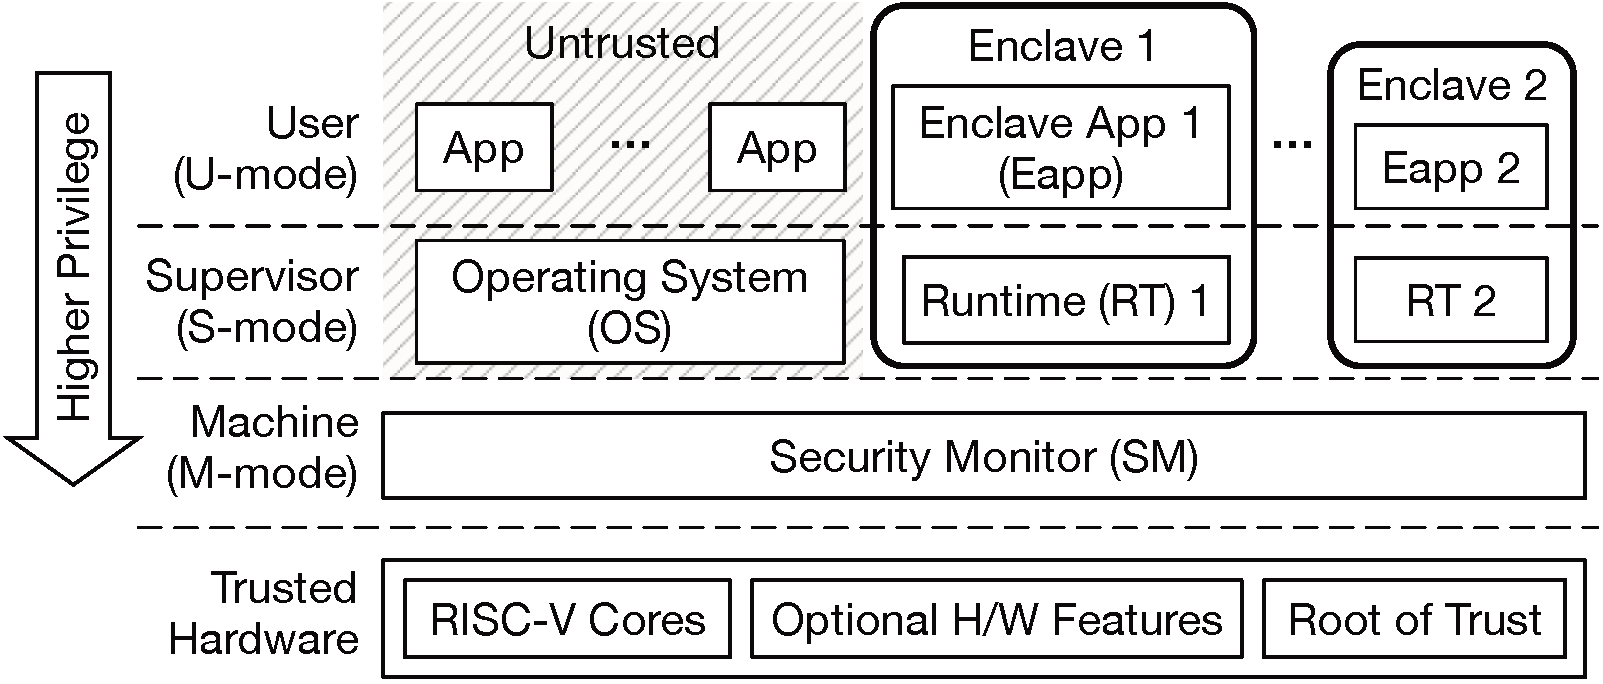
\includegraphics[width=0.8\linewidth]{img/keystone_overview.png}
    \caption{Keystone overview (2.2.1 \cite{keystone-docs})}
    \label{fig:keystone-overview}
\end{figure}

The keystone environment is made of several, unequal and concurrent, components.
The diagram shown in figure \ref{fig:keystone-overview} highlights a privilege hierarchy, going from most to least privileged:
\begin{itemize}
    \item Trusted Hardware: That is composed of \textit{supposedly} trustworthy and contains RISC-V standards cores compatible with Keystone and a Root of Trust (for the SM machine).
    This part can also bring optional features working with memory (cache partitioning, encryption, cryptographic randomness, etc.). 
    For these features to be usable, the SM requires platform specific plug-ins (FU540 for example).    
    \item M-mode: The SM, with a small TCB is the communication between the OS and the Enclaves.
    \item S-mode: Composed mainly of the OS and then each RunTime (RT) part of enclaves are all separated to preserve isolation. The RT part of the enclaves manage all the system call, interruptions, memory managment and traps. the  
    \item U-mode: Is composed of all the untrusted apps (supervised by the OS) of the computer and all the Eapp part of the enclaves. Note that the enclaves, even in this mode, are encapsulated
\end{itemize}

\subsection{Workflow}
\begin{figure}[H]
    \centering
    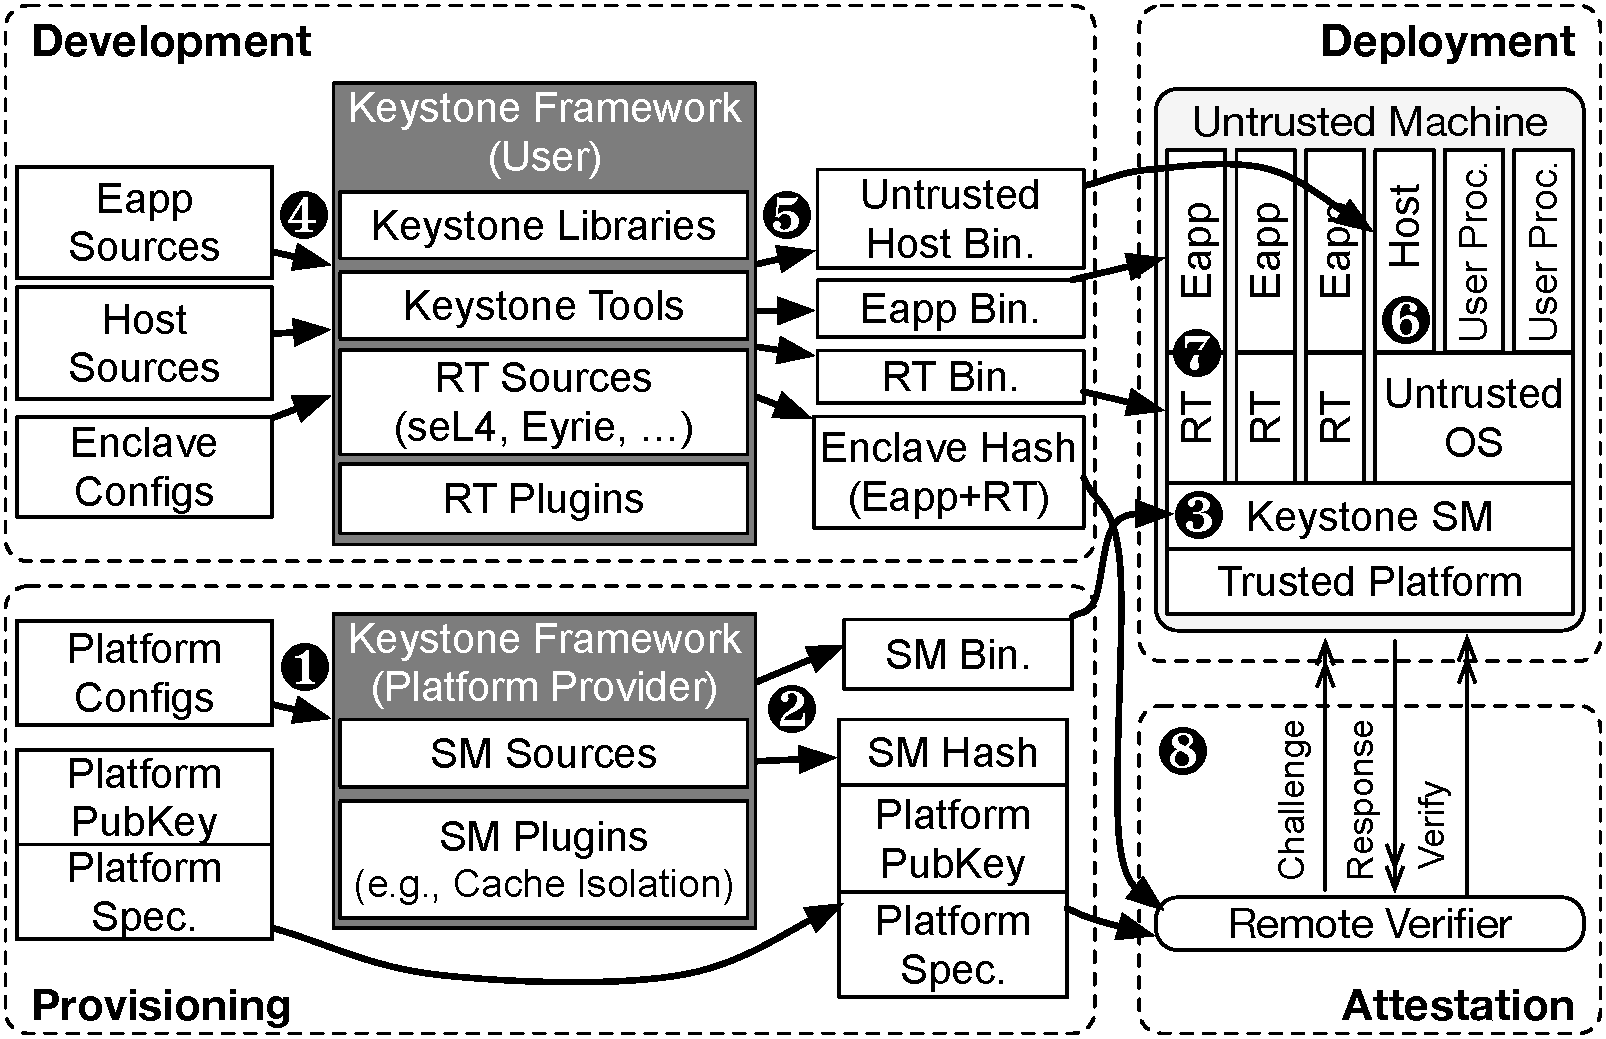
\includegraphics[width=0.8\linewidth]{img/keystone_workflow.png}
    \caption{Keystone workflow (2.2.2 \cite{keystone-web})}
    \label{fig:keystone-workflow}
\end{figure}

Keystone is a two-way framework. 
It is customizable by both the developers (of the enclaves) and by the platform producers. 
This means that building on it works in two different ways.
The former is the one that is in our interest. 
Even more, the need to develop a host "supervisor" of the enclave and interface to keep track inbetween runs will add a step.
\\

The basic workflow os to build de the eapps, the host and then \textit{possibly modified} runtime binaries.
Then, they can (but don't have to), be packaged together into a file (4,5).
The files are then deployed (6,7) into the remote system.
\\

Keystone also allows the enclaves to do a remote attestation (2.2.2.3. \cite{keystone-docs}).




\section{Enclaves}
\subsection{Enclave lifecycle}
\begin{figure}[H]
    \centering
    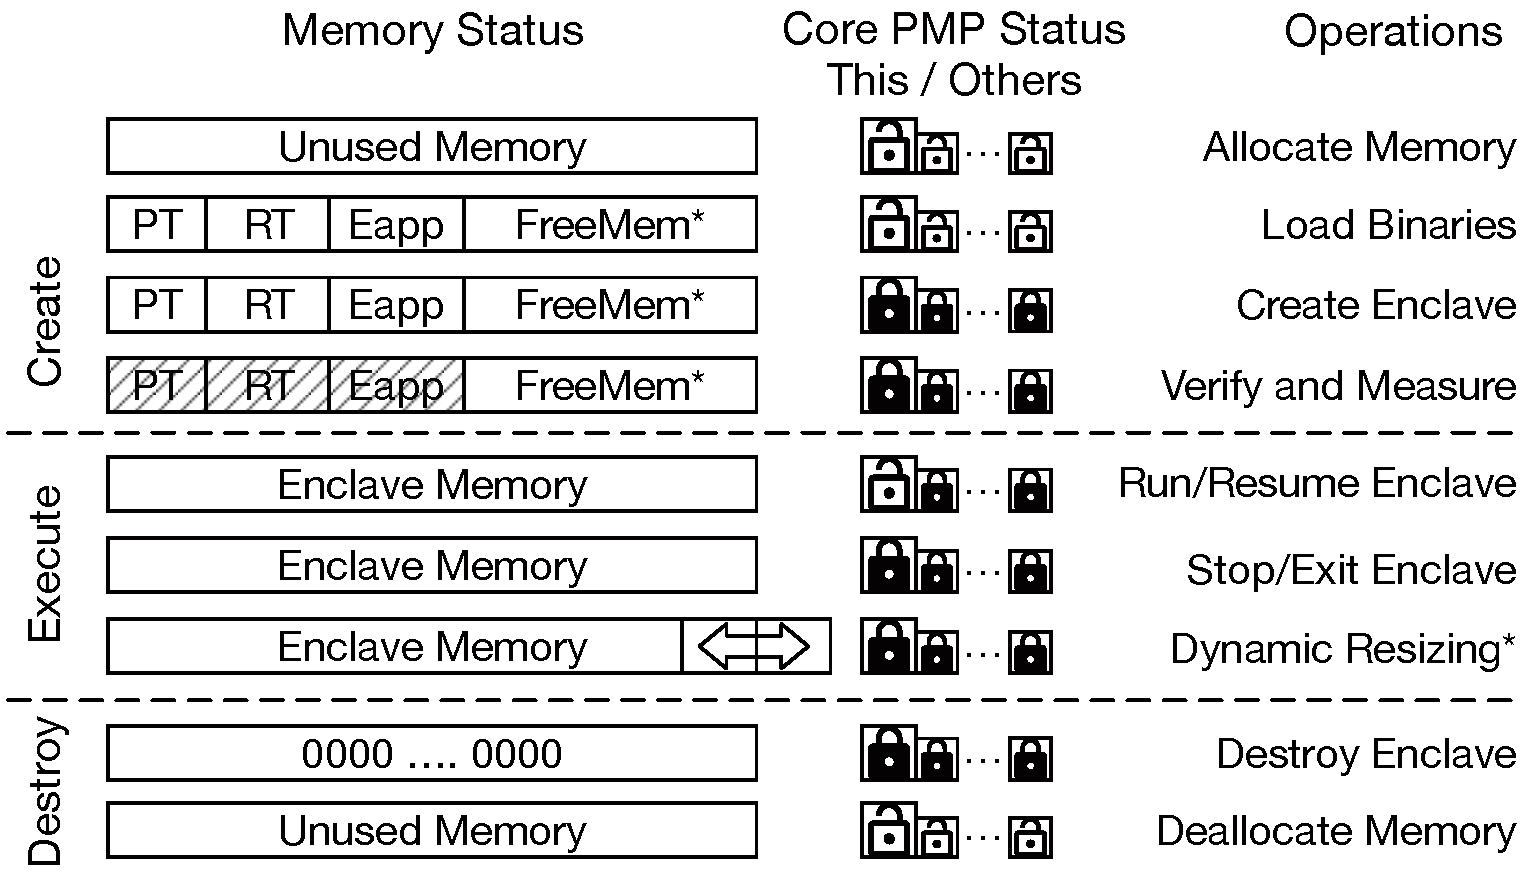
\includegraphics[width=0.8\linewidth]{img/enclave_lifecycle.png}
    \caption{Enclave overall lifecycle (2.2.3 \cite{keystone-docs})}
    \label{fig:enclave-lifecycle}
\end{figure}

\begin{figure}[H]
    \centering
    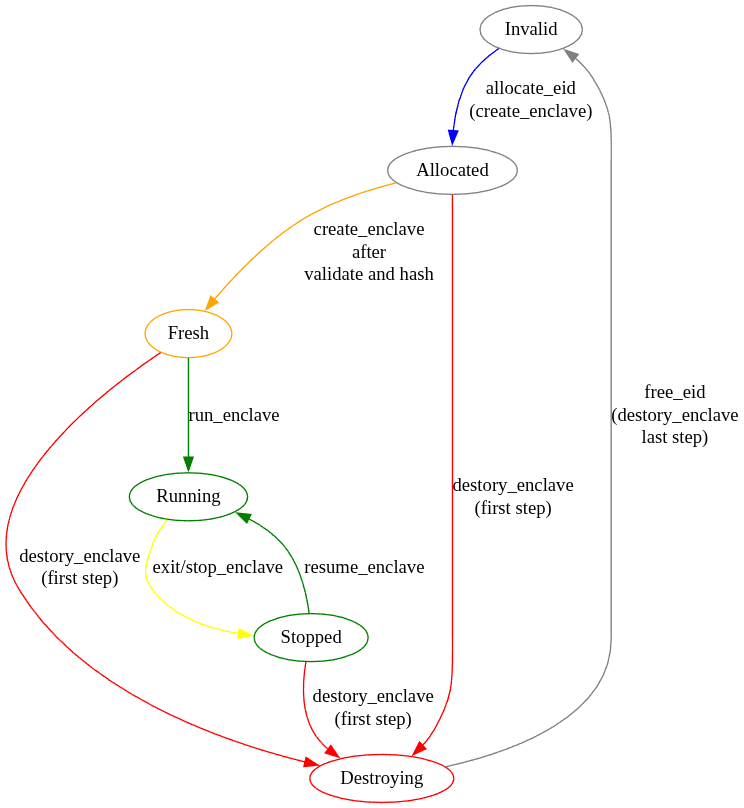
\includegraphics[width=0.5\linewidth]{img/diagram_lifecycle.png}
    \caption{Current Enclave Lifecycle (1.9. Keystone Security Monitor\cite{keystone-docs})}
    \label{fig:current-enclave-lifecycle}
\end{figure}

There are three main states for the enclave to be in ((2.2.3) \cite{keystone-docs}):
\begin{itemize}
    \item \textbf{Creation}: The (untrusted) host calls the SM with the Enclave Private Memory (EPM) allocated and the enclave's Page Table (PT).
    The SM then receives the host's call and encapsulate the EPM using a PMP entry.
    The entry is then shared among the cores so that the EPM is sealed from other cores.
    The SM then checks, right before execution, the state of the enclave (in case of an error). 

    \item \textbf{Execution}: Still on the host side, it makes a call to the SM. This time to execute the enclave and passing it to on of the SM's core.
    The SM thus relieves a PMP entry and the execution starts.
    The enclave can be exited and resumed at any time in the execution. Each time the PMP permission is switched to maintain isolation.
    
    \item \textbf{Destruction}: As well as exiting and resuming the enclave, the host can destroy it.
    For that, the host calls the SM. the later clears the EPM and then relieve the PMP entry.
    Last step is for the host to reclaim the newly available memory. 
     
\end{itemize}

\section{Quick EMUlator (QEMU)}
\label{sub:qemu}
QEMU is a free and open-source emulator and vizualizer \cite{qemu-website}. 
It has three different operating modes:
\begin{itemize}
    \item The user emulation that runs a single program.
    \item The system emulation which emulates a (and possibly several) full system, including preipherals and different architectures like RISC-V. 
    This is the mode used for Keystone. 
    \item The hypervisor support to act as a virtual-machine manager (VMM) or a backend emulation-device for virtual machines.
\end{itemize} 

\subsection{Eyrie runtime}
\label{sub:eyrie}
Eyrie is Keystone’s reference enclave runtime, it runs inside the enclave in trusted mode, manages memory and basic system-calls.
It sits between the enclave Eapp and the SM interface \cite{Eyrie, review-keystone}.
The module is not a submodule of Keystone, this allows modularity and force manual updates \cite{keystone-docs}. 

\subsection{FireSim}
"FireSim is an FPGA-based cycle-accurate simulator for RISC-V processors. 
Using FireSim, you can test Keystone on open-source processors" (1.2.2 \cite{keystone-docs}).
It is an alternative run (for Keystone's usage) to QEMU as it simulates the hardware \cite{FireSim}.

\section{Edge calls}
\label{sub:edge-calls}
An Edge call is a function that enters or exits the system. 
A visual representation is that it is at the \textit{edge} of it, meaning that the method goes from inside to outside and the other way around.
\\

In Keystone, it is used to communicate between the host (unsafe) and the enclave (safe). 
This is accomplished using shared memory between the two. 
More precisely using Outbound CALLs (\texttt{OCALL}). However, this is done by using offsets in memory region, using solely offsets (neglecting virtual address pointers)
\cite{keystone-docs, review-keystone}.

\subsection{OCALL lifecycle}
To make things clear, we'll use an example of usage. 
If we want to print something from inside the enclave, we need to : 

\begin{itemize}
    \item First, decide, with the host (at implemtation time), for the edge call corresponding to print: \texttt{OCALL\_PRINT\_VALUE}. 
    \item Next, stock the value input \texttt{val} ($enclave\rightarrow host$) we want to print.
    \item Optional, we decide of a return buffer value \texttt{ret} ($host \rightarrow enclave$).
    \item Now make the \texttt{OCALL}: \\
    \texttt{ocall(OCALL\_PRINT\_VALUE, \&val, sizeof(val), }\\
    \texttt{\&ret, sizeof(ret))}
\end{itemize}

Now the runtime part allocates an \texttt{edge\_call\_t} structure in shared memory. 
Then fills the call type and copies the value in the another part of the shared memory using an offset.
The last part for the enclave now is for the runtime to exit the enclave without destroying it. 
This is done with an \texttt{SBI\_CALL} expressing an ocall.
\\
Now the kernel resumes, checks for the enclave and sees a pending ocall. 
The execution is thus passed to the host.
The host read the \texttt{edge\_call\_t} (destroying it at the same time) and notice that it is \texttt{OCALL\_PRINT\_VALUE}.
The host then uses the same offset to read the buffered value and calls \texttt{\_print\_value} with the previously read value as an argument.
After that, as for the enclave call, the \texttt{ret} buffer can be filled (if it was not 0 in the original ocall) with with data in the shared memory.
The \texttt{edge\_call\_t} status is set to \texttt{SUCCESS} and the edge call is done for the host.
\\

An \texttt{SBI\_CALL} is emitted and the runtime re-enters the enclave. 
The runtime checks for a returned value (if the return buffer wa not 0 at the start). 
If so, it then uses the offset to put the data in \texttt{ret} and then resumes the wrapper code and passes any return value to the first ocall function.
\\

Note that this can also be used to provide networking operations \cite{review-keystone}.
\\

Since the implementation is assymetric, the host will have to map the edge calls that it could receive to wrapper functions and be able to handle them while running the main loop.
The enclave with just send the \verb|OCALLs| and wait for a possible response from the host.

\subsubsection{Host-side}
\label{subsub:edge-call-host}
The edge call wrappers are working in parallel to the main loop.
These wrappers are implemented as such:
\begin{verbatim}
// 1. Linking the edge calls to the functions
// this is done in configure_enclave()

// binds ocalls to the enclave 
enclave.registerOcallDispatch(incoming_call_dispatch); 
register_call(OCALL_PRINT_BUFFER, 
            print_buffer_dispatch); // input
register_call(OCALL_SAVE_CHECKPOINT_BLOB, 
            save_checkpoint_blob_dispatch); // input
register_call(OCALL_LOAD_CHECKPOINT_BLOB, 
            load_checkpoint_blob_dispatch); // output

// 2. Basic edge call structure
void edge_call_wrapper(void *buffer) 
{

    // 3. Checks the call sanity  
    if (edge_call_args_ptr(edge_call, &arg_ptr, &arg_size) != 0 
        || arg_size == 0) 
    {
        edge_call->return_data.call_status = CALL_STATUS_ERROR;
        return;
    }

    /* 4. Wrapper logic */ 

    // 5. Setup return data
    ret_val = /* some logic */
    uintptr_t data_section = edge_call_data_ptr();
    memcpy((void*)data_section, 
            &ret_val, 
            sizeof(type_to_return));
            
    if (edge_call_setup_ret(edge_call, 
                            (void*)data_section, 
                            sizeof(type_to_return))) 
    {
        call_status = CALL_STATUS_BAD_PTR;
    }

    // 6. Exiting
    edge_call->return_data.call_status = call_status;
    return;

}
\end{verbatim}

\subsubsection{Enclave-side}
\label{subsub:edge-call-eapp}
In contrast to the host, the edge calls in the enclave are sequential and in the main loop.
\begin{verbatim}
// The edge functions are :
// output
int save_checkpoint(uintptr_t stack_anchor, size_t anchor_len);
unsigned long ocall_print_buffer(char* data, size_t data_len);

// input
int load_checkpoint(struct rewind_checkpoint *checkpoint);


// 1. Basic edge call wrapper structure
auto edge_call_wrapper(int argc, char** argv) 
{   
    // 2. OUTPUT functions
    {    
        /* output wrapper logic */
    }

    // 3. OCALL
    auto retval;
    ocall(OCALL_ENUM_NUMBER, 
            data, 
            data_len, 
            &retval, 
            sizeof(retval));

    // 4. INPUT functions
    {
        /* input wrapper logic */
    }

    //5. Exit
    return (output ? retvall : some_value);
    
}
\end{verbatim}
Note that no standard library is used in the enclave as the Keystone tutorial (7.1.1 \cite{keystone-web}) explicitly states that printf is not a secure I/O interface.
Considering this, small functions to format numbers into strings (char*) have been implemented.


\section{Data sealing}
\label{sec:data-sealing}
Keystone has a sealing protocol. 
Using this, an enclave can save data in an untrusted, non-volatile, memory outside of its memory range.
It works by enabling the SM to to compute a \texttt{deterministic key} from the RoT for the enclave to use.
The key works both for sealing and unsealing data.
The deterministic operation is based on the device, a given enclave and a given SM running on a given processor will always yield the same key. 
Therefore, a combination including any differing component will give a different key \cite{keystone-docs, review-keystone}.
\\

A simple example of usage is given in the github repository (\keystonegithub)
at \texttt{examples/tests/data-sealing/data-sealing.c}:
\begin{verbatim}
char *key_identifier = "identifier";
struct sealing_key key_buffer;
int ret = 0;

/* Derive the sealing key */
ret = get_sealing_key(&key_buffer, sizeof(key_buffer),
                    (void *)key_identifier, 
                    strlen(key_identifier));

\end{verbatim}
This snippet is implemented in the enclave side. 
Note that there is an \textit{identifier} \label{def:key-identifier}, this allows the enclave to ask for several keys.
Each of them are unique (and deterministic) for a given identifier. 
\\

Another subroutine for an enclave is to ask for an attestation using an SBI call \texttt{attest} that can be passed to the host using an edge call.
The SM will generate and sign an attestation for the enclave.
More informations about this can be found in the documentation at \textit{5. Attestation} \cite{keystone-docs}.

\subsection{Key-Hierarchy}
\label{sub:key-hierarchy}
\begin{figure}[H]
    \centering
    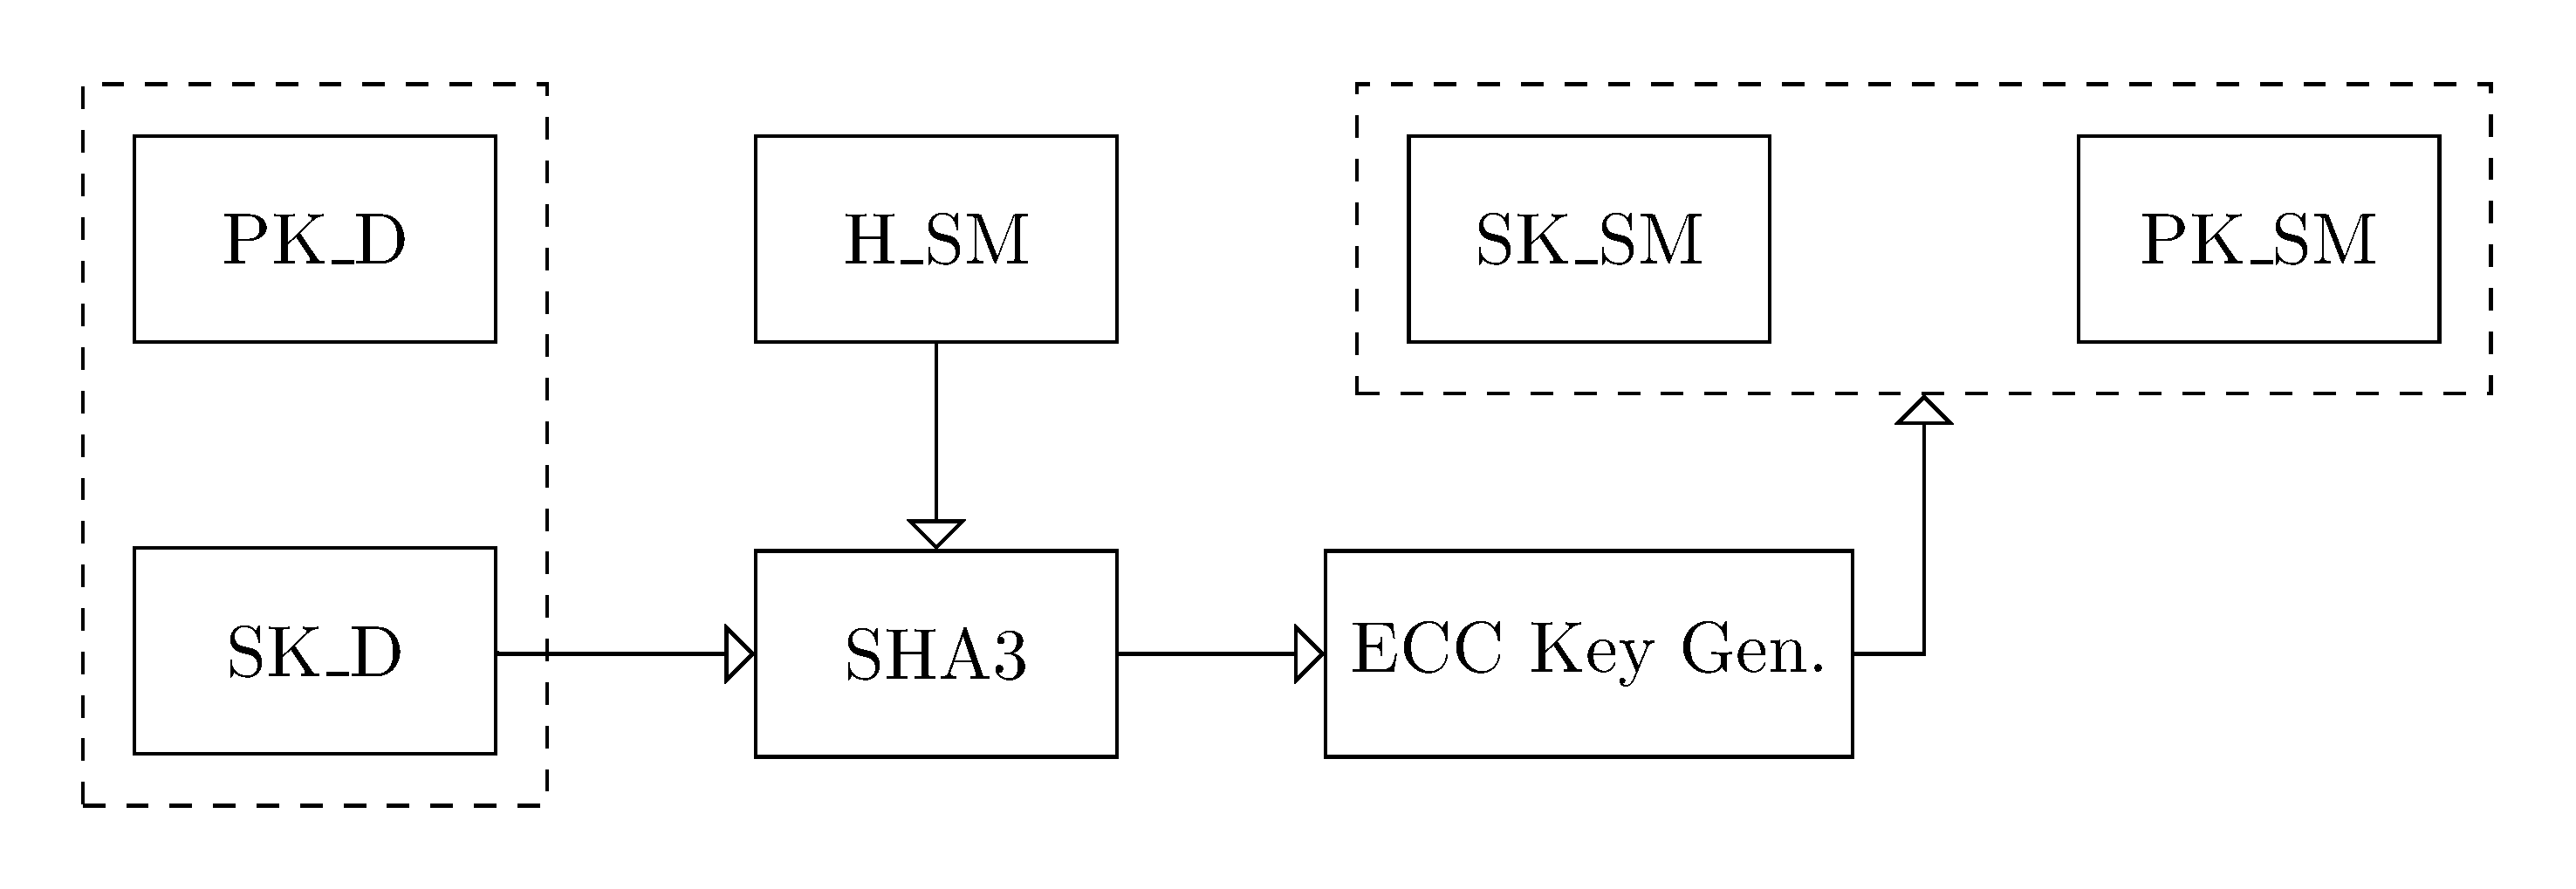
\includegraphics[width=0.8\linewidth]{img/keystone_key_hierarchy.png}
    \caption{Key-Hierarchy (6.1. Keystone Key-Hierarchy \cite{keystone-docs})}
    \label{fig:key-hierarchy}
\end{figure}
The base of this hierarchy is at the left-most. This is the asymetric key pair (public and private) of the processor (\texttt{PK\_D, SK\_D}).
Computing the private key with the SM hash (\texttt{H\_SM}) which is derived from the RoT in SHA3. 
Thus, as long as the RoT is safe, so is the SM's measurments.
The result of the computation is used as a scalar for the Elliptic-Curve Cryptography (ECC) Key Generator.
The final reslt is another key pair. This is the SM key pair (\texttt{PK\_SM, SK\_SM}).

\subsection{Key Derivation}
\begin{figure}[H]
    \centering
    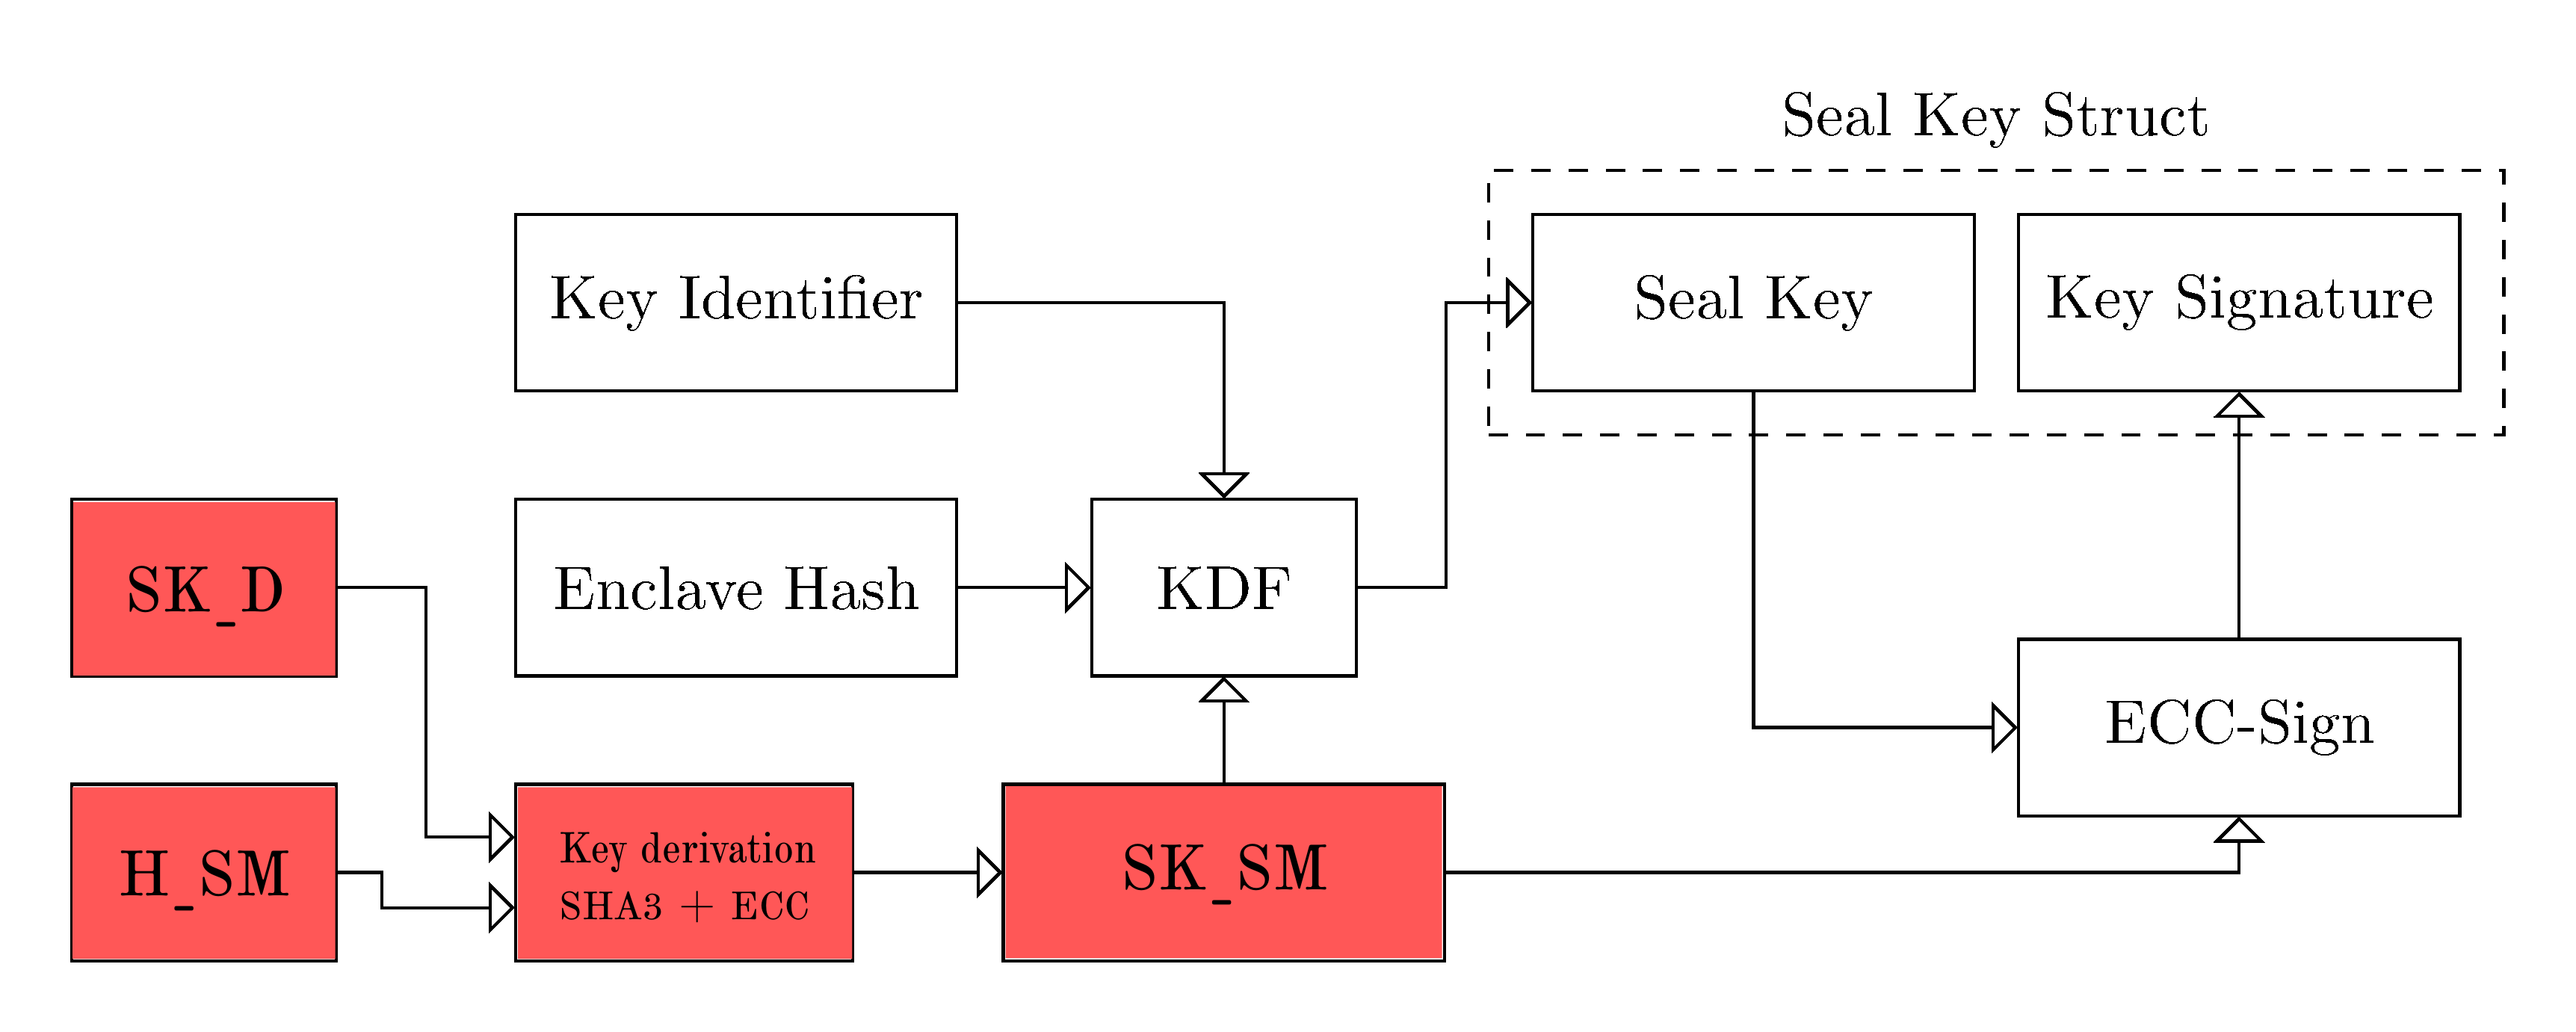
\includegraphics[width=0.8\linewidth]{img/sealing_key_deriv.png}
    \caption{Key Derivation Diagram (6.2 Sealing-Key Derivation \cite{keystone-docs})}
    \label{fig:sealing-key}
\end{figure}
The red blocks are what we already computed in the Key Hierarchy \ref{sub:key-hierarchy} subsection.
\\

Now that the SM has a key pair, it can derive keys for the enclaves.
This is done using three components:
\begin{itemize}
    \item \texttt{SK\_SM}: SM private key, it ensures that the key is bounder to the SM (and thus the RoT).
    \item The Enclave Hash, it ensures that the key is bounded to the enclave.
    \item A \textit{key Identifier} (\ref{def:key-identifier}), it is an additionnal input for the enclave to be able to derive multiple keys.
\end{itemize}
The three components are computed in a Key Derivation Function (KDF). 
The resulting sealing key is then signed using ECC and then placed in the Seal Key Struct (implemented as \texttt{sealing\_key}):
\begin{verbatim}
struct sealing_key {
    uint8_t key[SEALING_KEY_LENGTH];
    uint8_t signature[SIGNATURE_SIZE];
};    
\end{verbatim}


\section{Compilation}
\label{sub:compilation}
As shown in the documentation, compilation in Keystone is, at first sight, a simple task (1.2.1.3. Compile Sources \cite{keystone-docs}).
However, all of its different, standalone, components (\ref{sub:eyrie}, \ref{sub:qemu}) make it  very modular and thus more complex.

The basic command to compile the source files is:\\
\begin{center}
\verb|make -j$(nproc)|
\end{center}
This is divided in 3 different parts:
\begin{itemize}
    \item \verb|make|: Runs the \verb|Makefile|.
    \item \verb|-jN|: "Specifies the number of jobs (commands) to run simultaneously." - Manual page Ubuntu 20.04
    \item \verb|$(nproc)|: the \verb|$()| is a shell substitution for the \verb|N|, the output of the \verb|nproc| command gives the number of available processing units and is placed in the \verb|$()| substitution.
\end{itemize}
All together, the Makefile is executed using all the available processing units.
This will build all the components and generate a bootable image, the output build in \verb|build-$PLATFORM$BITS|.
\\

Also, there are possible options for it, these options are given below (presented with the default parameter) and can be given in the terminal using: 
\begin{center}
\verb|OPTION1=VALUE1 OPTION2=VALUE2 (...) make -j$(nproc)|
\end{center}

\subsection{Rebuilding Changed Components}
We can include specific directories to be cleaned in order to avoid stale sources:
\begin{center}
\verb|BUILDROOT_TARGET=<target>-dirclean|
\end{center}
The new part is the targeted directory (\verb|<target>|),
this could be :
\begin{itemize}
    \item \verb|keystone-examples|
    \item \verb|keystone-sm|
    \item \verb|keystone-runtime|
    \item \verb|all|
    \item etc.
\end{itemize}
When the compiler notices a stale, a warning message will be shown :
\begin{verbatim}
>>>  (WRN) Stale build directory detected for keystone-examples! 
>>>  (WRN) You should build keystone-examples-dirclean to remove them. 
>>>  (WRN) Not doing so may leave your build in an inconsistent state.
\end{verbatim}
For this example, the following build command should be ran:
\begin{center}
\verb|BUILDROOT_TARGET=keystone-examples-dirclean make -j$(nproc)|
\end{center}


\subsection{Platform}
We can configures the platform to build. 
The default is \verb|generic| and only supports qemu \ref{sub:qemu}.
\begin{center}
\verb|KEYSTONE_PLATFORM=generic|
\end{center}


\subsection{Bits}
We can choose either RV32 or RV64.
\begin{center}
\verb|KEYSTONE_BITS=64|    
\end{center}


\subsection{Builroot Config file}
Sets the configuration file for the buildroot to use.
\begin{center}
\verb|BUILDROOT_CONFIGFILE=qemu_riscv$(KEYSTONE_BITS)_virt_defconfig|
\end{center}





%%%%%%%%%%%%%%%%%%%%%%%% System Model %%%%%%%%%%%%%%%%%%%%%%%%
\chapter{System Model and Design}
This chapter describes the concrete implementation, the choices and the assumptions that have been made.

\section{Preliminary setup and selection}
The first step is to have a strong, yet modular, idea of the concept to be implemented.
The goal is to obtain domains that can be checkpointed and the data that has been sealed needes to be accessible in another one.
The domains discussed here are the ones from the "Rewind $\&$ Discard: Improving Software Resilience using Isolated Domains" \cite{sdrad}.
We can make an easy parallel between enclaves and domains as they are executed in an isolated execution context with controlled memory (\ref{sub:pmp}) from the outer, untrusted, world.
The SM (\ref{sub:sm}) is an enclave factory and provides them with, as previously mentionned, controlled memory.

% data sealing
Furthermore, several enclaves of the same binary (compiled source file) can be initialized. 
This is important for the key generation of an enclave (\ref{sec:data-sealing}).
In the case of a fault occuring in an enclave, the host can see the return code of the enclave and ask for the SM to create another instance of that same enclave (using PMP entries).
The two instances will (as the key generation is determistic \cite{keystone-docs, review-keystone}) have the same resulting sealing key.
This is true if we consider the identifier to be the same for both, as it is implemented in the binary of the enclave's eapp, the statement is supposedly satisfied.

% data sealing & edge calls
For the checkpointing scheme, the enclave use the edge calls (\ref{sub:edge-calls}) already implemented in keystone. 
The checkpointed data is sent and retrieved (to and from the host's memory space) using the enclave's key trough two custom edge calls. 
To ensure that the data isn't tampered, there is a layer on top of Keystone's encryption scheme.
The layer adds a tag and an Initialisation Vector (IV) for the enclave to check if the unsealed data corresponds to the sealed one.
Only the last checkpoint is saved.

In this project, there is only one binary source (the compile code) and it doesn't implement any fault assessment, the enclave behaves as if the fault caused a fatal crash and stops immediatly, returning an error.
One possible fallback would be to use a degraded version of the enclave in order to prevent attacks using the computation power and overloading a server by making it fail a task idefinitly for example. 
We address this in the future work section \ref{sub:back-complexity}.

% Fault model
% Tests
\section{Threat Model}
\label{sec:threat-model}
A threat model helps to clarify the hypothesis, the goals and the limitiations compared to the real, unsafe, world. 
To this extent, we will ground the thesis over a specififed one.
\\  

First, the trusted domain. 
It consists of the enclave code, its runtime, and its memory access under Keystone, RISC-V, and PMP isolation. 
It also includes enclave-derived sealing keys, obtained through \texttt{get\_sealing\_key}, because these keys are bound to the enclave measurement.

Second, the adversarial domain. 
This includes the \textbf{host}, the OS, and everything outside the enclave, with an exception for the \textit{SM}, \textit{RoT} and \textit{PMP entries} that run the said enclave. 
It also includes the channel carrying the sealed blob, whether that channel is host storage, an OCALL buffer, or any other transport. 
Finally, it includes physical disruption such as power loss \cite{sdrad, ARM-TrustZone-CortexM}, since an attacker may trigger crashes or power cuts.

Next, the attacker capabilities. 
It can read, write, replay, or corrupt any sealed blob stored on the host. 
It can also trigger enclave stops, or even destruction, when incoming edge calls arrive, and it can crash power or execution at arbitrary points.

After that, the security objectives. 
They are confidentiality, integrity and authenticity, atomicity, and unclonability. 
Confidentiality requires the checkpoint contents to remain unreadable to the host. 
Integrity and authenticity require that a tampered blob is detected and rejected without leaking information through response time analysis. 
Atomicity requires that no undefined state can arise from interrupted checkpoint writes. 
Unclonability requires that the device cannot be cloned from checkpoint data alone.

Finaly, the accepted limitations. 
These are replaying and rollback are out of scope because the host is the only link to the outside world and cannot be trusted.
Edge call manipulation, such as enclave stall or destruction, is also out of scope for the same reason.

\subsection{Assumptions}
The attacker may obtain arbitrary access to process (host) memory and may trigger run-time attacks that corrupt application state, but cannot modify code pages of the enclave under a W\(\oplus\)X policy \cite{sdrad, security-privacy}. 
The attacker is also assumed to detect or exploit software-level vulnerabilities, while transient execution attacks, hardware-level fault injection, and other hardware or firmware-level attacks are out of scope and assumed to be covered by the Keystone security implementation. 
In the Keystone setting, we additionally assume the enclave isolation and the underlying secure world mechanisms protect enclave code and secrets against direct software manipulation, and that the host is not trusted with enclave state recovery details.

We further assume that the checkpointing and rewind mechanism operates securely, that is: a state external to the protected domain may be compromised, but the protected recovery boundary must remain trustworthy. 
For the intermittent-device context, the checkpointed state may be exposed to physical disruption such as power loss or tampering with external storage.
The enclave only restores the checkpoint on restart and does not base its execution on the sealed checkpoint it sent unless there is a fault and thus a, possibly corrupted, rewind.

Enclave execution is assumed deterministic given identical entry state (no host-controlled inputs, per Attacker Capabilities). Under this assumption, IV/seq reuse acrosscrash-and-restart is safe: identical plaintext re-encrypted under the same IV leaks nothing.
This safety does not hold if the enclave itself introduces non-determinism (uninitializedmemory, internal RNG/timer reads, etc.) before the point of divergence from a prior checkpoint\_seq.

\subsection{Requirements}
The system must allow the application to continue operation after a detected fault or attack by restoring a trusted state and resuming execution from a safe point. 
The recovery mechanism must preserve memory integrity after rewind, and isolation must ensure that faults in one compartment do not compromise other protected compartments or the logic responsible for transitions and recovery.

An enclave state must remain protected across enclave transitions, that recovery metadata must be authenticated, and that the host must not be able to forge or tamper with a checkpoint without detection.



\section{Implementation}
So far, this thesis has mainly covered concepts \ref{chap:SotA}, ground work \cite{ARM-TrustZone-CortexM, sdrad, keystone-repo} and limitiations.
All of these are used to produce the implementation of the rewind enclave mechanism.
\\

The files that are implemented and described can be found on the \github.
Also note that the repository setup is described at the end of the \verb|README.md| (at the root of the repository itself).
All of these files are also available in the Appendix \ref{chap:appendix}. 
\\

Implementing the rewind example is done in two different places, the \verb|eapp/| and \verb|host| subfolders.
The eapp is, as shown is the Keystone Basics \ref{sub:basics}, the trusted part and would be considered a \textit{transient domain} \cite{sdrad}.
A transient domain can exit (abnormally or not), it doesn't retain data upon exiting and is closed from the outer world (in both writing and reading).
In comparison, the host would be considered a \textit{persistent domain} as it keeps the enclave data (the sealed checkpoint), it cannot look into an enclave's memory region (except for the shared one given by the SM).
However, the host is \textbf{not} trusted in itself.

To address this security issue, the checkpoint is sealed (using the sealing key provided by the SM) and uses a tag. 
This ensure that the host can neither read it or tamper with it.
Upon unsealing a the checkpoint, the enclave checks its tag so see if it fits the data. 
If not, the  data is discarded and the enclave restarts the computation from the beginning.

The discard and rewind is done by asking the SM to destroy the enclave, free the PMP entry and then allocate a new entry on the the same binary to create the rewinded version of the enclave.
This new enclave's instance will ask the host (using and edge call) for any saved, sealed, checkpoint. 
If the host has one it will copy the blob in the shared memory region and the enclave will consume it to try and restore the last checkpoint.
If not, the enclave will start from scratch.
Note that the first enclave also does this protocol (as the same code is being used).

\subsubsection{Host-side}
There is only one execution changing macro, other setups are the edge calls :
\begin{itemize}
    \item \verb|MAX_RUNS|: Decides how many tries the host should do before stopping and considering the job failed.
    \item \verb|OCALL_PRINT_BUFFER = 1|: Links the OCALL $1$ to the print (input) wrapper.
    \item \verb|OCALL_LOAD_CHECKPOINT_BLOB = 8|: Links the OCALL $8$ to the load checkpoint (output) wrapper.
    \item \verb|OCALL_SAVE_CHECKPOINT_BLOB = 9|: Links the OCALL $9$ to the save checkpoint (input) wrapper.
\end{itemize}
The rewinding protocol in the \verb|host.cpp/.hpp| file \ref{file:host} looks like:
\begin{verbatim}
// 1. setup :
//  - the macros in the CMakeList 
//  - the edge calls number to be mapped

// 2. Setup the enclave parameters (memory-wise)
Params params;
uintptr_t ret = 1;
auto retry_counter = 0;

// 3. Beginning the execution loop
while (ret != 0  && retry_counter < MAX_RUNS) 
{

    // 3a. Configure the enclave
    // enclave.init() && linking edge calls to 
    configure_enclave(enclave, params, argv); 

    //SM destroy the enclave upon completion
    enclave.run(&ret); 
}

// 4. Exiting
return ret;
\end{verbatim}
The basic edge call wrapper structure is explained in the edge call section of the keystone architecture \ref{subsub:edge-call-host}.
The actual implementation of each wrapper is detailed in \ref{subsub:checkpoint-host}.

\subsubsection{Enclave-side (EAPP)}
As for the host, there is only execution changing macro, other setups are the (same) edge calls.
Note that the edge calls must be the same for the host and enclave in order to efficiently communicate.
\begin{itemize}
    \item \verb|EAPP_RUNS|: Decides how many iterations the enclave should do before stopping and considering the job done.
    \item \verb|OCALL_PRINT_BUFFER = 1| output
    \item \verb|OCALL_SAVE_CHECKPOINT_BLOB = 9| output
    \item \verb|OCALL_LOAD_CHECKPOINT_BLOB = 8| input

\end{itemize}
The rewinding protocol in the \verb|rewind.c| file \ref{file:rewind} looks like:
\begin{verbatim}
// 1. Setup :
//  - the macros in the CMakeList 
//  - the edge calls number to be mapped

// 2. Load the structs
struct rewind_state state = {0, 1, 0}; // a, b, counter
struct rewind_checkpoint checkpoint;
struct fault_model f_m = get_default_model();

// 2a. check for an existing checkpoint save
if (load_checkpoint(&checkpoint) == 0) 
{
    // 2b. try and restore the saved checkpoint if there is one 
    restore_checkpoint(&state, &checkpoint)
}

// 3. Beginning the execution loop
for (; state.counter < EAPP_RUNS;)
{

    // Fault happens before the end of the computation 
    // to mimic stall in the process.
    if (fault_should_trigger(&f_m)) 
    {
        // More explanations in Fault section
        EAPP_RETURN(16); 
    }

    // Fibonacci
    auto next = state.a + state.b;
    state.a = state.b;
    state.b = next;
    state.counter++;

    save_checkpoint((uintptr_t)&state, sizeof(state));
}

// 4. Exiting
EAPP_RETURN(0);
\end{verbatim}

\subsection{Checkpoint}
In order to rewind or discard an enclave, there must be a checkpointed state that is saved and loaded on demand (by the enclave, as defined by Keystone \ref{chap:Keystone}).
as for the overall implementation, the two sides have their own wrapper logic as they have an asymmetric relationship.
The host supervises the enclave and the latter is, once running, sealed from the former \ref{file:checkpoint}.
However, as soon as the enclave submit an edge call, the host could (assuming malicious intentions) destroy the enclave or stall it indefinetly.
This is bounded by Keystone structure and is, as noted in the threat model \ref{sec:threat-model}, not in the scope of this thesis.
\\

One could implement a direct call from the enclave to the SM to external safe memory with, for example, table pages protected by outside PMP entry or another "data enclave" that has a direct communication channel with the "runtime" one.
The problem in our scenario is that the host is the only link to the outside world and is, by definition, also not to be trusted.
This limitation being addressed, the saved checkpoint must be sealed and must be checked in order to not introduce unsafe data into the enclave's memory.


\subsubsection{Host-side}
\label{subsub:checkpoint-host}
The print buffer will not be detailed as it is already implemented in the Keystone basic examples and is thus already explained in the documentation \cite{keystone-web}.
Furthermore, the host keeps the last saved checkpoint blob in the \verb|inline vector<uint8_t> saved_blob| variable.
This will be used for both loading and saving.
\\

Notice that this variable, is one of the possible attack vectors for a malicious program that would corrupt the host (in both reading and writing).
The edge calls are, by definition and because they are linked to a specific function, another attack vector.

\paragraph{1. load wrapper}
\begin{verbatim}
void load_checkpoint_blob_dispatch(void* buffer)
{   
    // 1a. gather OCLL parameters
    struct edge_call* ecall = (struct edge_call*)buffer;

    // 1b. checks if there is a saved checkpoint
    if (saved_blob.empty()) 
    {
        ecall->return_data.call_status = CALL_STATUS_ERROR;
        return;
    }

    // 1c. looks into shared memory
    void* ret_buffer = (void*)edge_call_data_ptr();

    // 1d. save it
    memcpy(ret_buffer, saved_blob.data(), saved_blob.size());

    /* 1e. if TESTING enabled -> tamper */
    if (HOST_TESTING)
    {    
        tamper_checkpoint_blob(saved_blob);
    }

    // 1f. return and exit with ok status
    edge_call_setup_ret(ecall, ret_buffer, saved_blob.size());
    ecall->return_data.call_status = CALL_STATUS_OK;
}


\end{verbatim}

\paragraph{2. save wrapper}
\begin{verbatim}
void save_checkpoint_blob_dispatch(void* buffer)
{
    // 2a. gather OCLL parameters
    struct edge_call* ecall = (struct edge_call*)buffer;
    uintptr_t arg_ptr;
    size_t arg_size;


    // 2b. check parameters sanity
    if (edge_call_args_ptr(ecall, &arg_ptr, &arg_size) != 0 ||
        arg_size == 0) 
    {
        ecall->return_data.call_status = CALL_STATUS_ERROR;
        return;
    }

    // 2c. save (sealed) checkpoint
    saved_blob.resize(arg_size);
    memcpy(saved_blob.data(), (void*)arg_ptr, arg_size);

    // 2d. exit
    ecall->return_data.call_status = CALL_STATUS_OK;
}
\end{verbatim}

\subsubsection{Enclave-side}
As for the host, the enclave must keep an anchor in order to be able to save/load a checkpoint.
This is \verb|extern struct rewind_state *state_anchor|.

\paragraph{1. load wrapper}
\begin{verbatim}
int load_checkpoint() 
{   
    // 1a. sends an OCALL to the SM
    if (ocall(OCALL_LOAD_CHECKPOINT_BLOB, 
            NULL,               // data to send
            0,                  // size of this NULL data
            &checkpoint_blob,   // data to retrieve
            sizeof(checkpoint_blob)) != 0)
    {
        eapp_print("No saved checkpoint");
        return -1;
    }

    // 1b. try to unseal the retrieved data
    if (open_checkpoint_blob(&checkpoint_storage, 
                        &checkpoint_blob) != 0)
    {
        return -1;
    }

    // 1c. increment sequence and exit
    /* 
    the sequence is incremented to mimic what would happend
    if the the enclave was at this iteration and just saved
    (the increment is done after the save).
    */ 
    checkpoint_storage.checkpoint_seq++; 
    return 0;
}

// Note: The enclave must then use
// restore_checkpoint() 
// to restore the decrypted checkpoint into the state_anchor
\end{verbatim}

\paragraph{2. save wrapper}
\begin{verbatim}
int save_checkpoint()
{
    // 2a. setup parameters
    uintptr_t stack_sp;
    uintptr_t stack_anchor;
    uintptr_t snapshot_sp;
    uintptr_t snapshot_end;
    size_t snapshot_len;
    struct checkpoint to_save;  // temporary built checkpoint

    // 2b. load and check the parameters
    if (state_anchor == NULL)
    {
        eapp_print("Invalid checkpoint anchor");
        return -1;
    }

    memset(&to_save, 0, sizeof(to_save));
    stack_sp = read_stack_pointer();
    stack_anchor = (uintptr_t)state_anchor;
    snapshot_end = stack_anchor + sizeof(*state_anchor);

    snapshot_sp = snapshot_end > STACK_SNAPSHOT_SIZE
        ? snapshot_end - STACK_SNAPSHOT_SIZE
        : stack_sp;

    // keep the snapshot aligned to the current stack
    if (snapshot_sp < stack_sp) {snapshot_sp = stack_sp;}

    if (snapshot_end < snapshot_sp)
    {
        eapp_print("Invalid snapshot anchor");
        return -1;
    }

    snapshot_len = snapshot_end - snapshot_sp;

    if (snapshot_len > STACK_SNAPSHOT_SIZE)
    {
        eapp_print("Stack snapshot too large");
        return -1;
    }

    // 2c. save the current data into the tmp variable
    to_save.checkpoint_seq = checkpoint_storage.checkpoint_seq;
    memset(to_save.stack_data, 0, sizeof(to_save.stack_data));
    memcpy(to_save.stack_data+(STACK_SNAPSHOT_SIZE-snapshot_len),
            (void *)snapshot_sp,
            snapshot_len);

    memset(&checkpoint_blob, 0, sizeof(checkpoint_blob));


    // 2d. seal blob
    if (seal_checkpoint_blob(&checkpoint_blob, &to_save) != 0)
    {
        return -1;
    }

    // 2e. output OCALL
    if (ocall(OCALL_SAVE_CHECKPOINT_BLOB, 
            &checkpoint_blob,   // data to save
            sizeof(checkpoint_blob), 
            NULL, 0) != 0)  // no data to wait from the host
    {
        eapp_print("failed to save checkpoint");
        return -1;
    }

    // 2f. increment checkpoint_seq and exit
    checkpoint_storage.checkpoint_seq++;
    return 0;
}
\end{verbatim}

\subsection{Data encryption}
To preserve the security objectives, the enclave implements a cryptographic protocol Appendix \ref{file:crypto}.
\\

The authentificaction and encryption keys are both derived using the function\\
\verb|derive_checkpoint_material()| usging Keystone \verb|get_sealing_key()| \ref{sec:data-sealing}.
This function is cached after the first usage as the keys will never be changed afterwards. The worklow can be described as such:
\paragraph{1. Save}
\begin{itemize}
    \item[a)] \texttt{derive\_checkpoint\_material()} asks the SM sealing API
    for key material bound to scheme label (\texttt{identifiers[]}).
    \item[b)] The returned material is two independent AES-256 keys:\\
        - \texttt{enc\_key} for confidentiality (CTR stream encryption)\\
        - \texttt{auth\_key} for integrity/authenticity (CBC-MAC)
    \item[c)] \texttt{encrypt\_stack(payload)} AES-CTR-encrypts the plaintext
    payload and the iv.
    \item[d)] \texttt{compute\_tag()} MACs the ciphertext checkpoint payload.
    \item[e)] The payload and tag are copied into the host-facing blob.
\end{itemize}

\begin{verbatim}
// 1a-b . Derive checkpoint key material
if (derive_checkpoint_material() != 0) { return -1; }

// 1c. encrypt_stack(payload): 
// AES-CTR-encrypt payload, build iv from checkpoint_seq
uint8_t iv[AES_BLOCK_SIZE] = {0};
memcpy(iv, 
    &checkpoint->checkpoint_seq, 
    sizeof(checkpoint->checkpoint_seq));
memcpy(iv + sizeof(checkpoint->checkpoint_seq), 
    &checkpoint->checkpoint_seq, 
    sizeof(checkpoint->checkpoint_seq));

uint8_t mac_input[AES_BLOCK_SIZE + 
                sizeof(struct checkpoint)];
size_t mac_len = AES_BLOCK_SIZE + payload_len;
memcpy(mac_input, iv, AES_BLOCK_SIZE);
memcpy(mac_input + AES_BLOCK_SIZE, payload, 
    payload_len);

                
aes_key_setup(enc_key, enc_schedule, AES_KEY_BITS);
aes_encrypt_ctr(mac_input, mac_len, 
            mac_input, 
            enc_schedule, 
            AES_KEY_BITS, 
            iv);

// 1d. compute_tag(): AES-256-CBC-MAC over the ciphertext and iv
uint8_t zero_iv[AES_BLOCK_SIZE] = {0};
aes_key_setup(auth_key, auth_schedule, AES_KEY_BITS);
aes_encrypt_cbc_mac(payload, payload_len, 
                    tag, 
                    auth_schedule, AES_KEY_BITS, 
                    zero_iv);

// 1e. Copy ciphertext payload, iv and tag into the blob
memcpy(blob->iv, iv, sizeof(iv));
memcpy(blob->sealed, payload, sizeof(payload));
memcpy(blob->sealed + sizeof(payload), tag, sizeof(tag));

// the blob is then sent to the host using the 
// previously described OCALL_SAVE_CHECKPOINT_BLOB edge call
\end{verbatim}


\paragraph{2. Load}
\begin{itemize}
    \item[a)] Derive the same \texttt{enc\_key}/\texttt{auth\_key} again from
    the same context.
    \item[b)] Split the opaque blob into ciphertext, iv, and tag.
    \item[c)] Recompute the expected tag over the ciphertext and given iv.
    \item[d)] Compare expected tag with the stored tag; if mismatch, reject.
    \item[e)] Decrypt the ciphertext.
    \item[f)] Rebuild the plain checkpoint.
\end{itemize}

\begin{verbatim}
// 2a. Derive the same enc_key/auth_key 
// again from the same context
if (derive_checkpoint_material() != 0) { return -1; }

// 2b. Split the opaque blob into ciphertext, iv, and tag
memcpy(iv, blob->iv, sizeof(iv));
memcpy(ciphertext, blob->sealed, sizeof(ciphertext));
memcpy(tag, blob->sealed + sizeof(ciphertext), sizeof(tag));

// 2c. Recompute the expected tag over the ciphertext
compute_tag(ciphertext, sizeof(ciphertext), expected_tag);

// 2d. Compare expected tag with the stored tag; 
// reject on mismatch
if (memcmp(expected_tag, tag, 
            sizeof(expected_tag)) != 0) {
    eapp_print("checkpoint authentication failed");
    return -1;
}

// 2e. Decrypt the ciphertext,
// same iv derived from checkpoint_seq
aes_key_setup(enc_key, enc_schedule, AES_KEY_BITS);
aes_decrypt_ctr(ciphertext, sizeof(ciphertext),  
                payload, 
                enc_schedule, AES_KEY_BITS, 
                iv);

// 2f. Copy the plain decrypted checkpoint 
memcpy(checkpoint, payload, sizeof(*checkpoint));
\end{verbatim}

\subsubsection{Data structures}
\label{subsub:data-struct}
Three data structures separate three distinct roles in the checkpoint/rewind
pipeline:

\begin{verbatim}
struct checkpoint checkpoint_storage
struct sealed_checkpoint checkpoint_blob
struct rewind_state *state_anchor
\end{verbatim}
The implementation size of the resulting blob can be seen by setting the macro (and the overall eapp tests)
\verb|EAPP_BLOB_SIZE_TESTING| to $1$.

\begin{table}[H]
    \centering
    \label{tab:seal_cp_size}
    \begin{tabular}{|l|r|}
        \hline
        Component & bytes \\
        \hline
        IV & 16 \\
        Plain text & 8208 \\
        Tag & 16 \\
        Total & 8240\\
        \hline
    \end{tabular}
    \caption{Sealed checkpoint size (bytes)}
\end{table}

\begin{itemize}
    \item \texttt{struct checkpoint checkpoint\_storage}: the
    \textit{plaintext} in-enclave representation of the saved state
    (e.g. register file, stack snapshot, sequence number). This is the
    object produced right before sealing and the object reconstructed
    right after unsealing. It never leaves the enclave in this form.

    \item \texttt{struct sealed\_checkpoint checkpoint\_blob}: the
    \textit{host-oriented, opaque} container holding the encrypted payload,
    the IV, and the authentication tag. This is the only representation
    of the checkpoint that is allowed to cross the enclave boundary and
    be stored/transmitted by the untrusted host.

    \item \texttt{struct rewind\_state *state\_anchor}: the
    \textit{runtime pointer/metadata} used by the rewind mechanism to
    locate and validate which checkpoint(s) are eligible for restoration
    (e.g. current sequence number, pointer to active checkpoint, rewind
    policy state). It is not itself sealed; it governs \textit{which}
    \texttt{checkpoint\_blob} may be opened and \textit{when}.
\end{itemize}

\paragraph{Cryptographic primitives and concepts.}
\begin{itemize}
    \item \textbf{CBC-MAC}: Message Authentication Code built by
    running block-cipher CBC encryption over the message and keeping
    only the final block as the tag. Provides integrity/authenticity,
    \textit{not} confidentiality. Secure only for fixed-length messages
    unless additional length-binding is used.

    \item \textbf{CTR (Counter mode)}: block-cipher mode that turns
    AES into a stream cipher by encrypting successive counter values
    and XOR-ing the result with plaintext/ciphertext. Provides
    confidentiality only; requires a unique \texttt{(IV, key)} pair per
    encryption to remain secure.

    \item \textbf{ENC / AUTH}: shorthand for the two independent
    purpose-bound keys derived from the sealing key material:
    \texttt{enc\_key} (used only for CTR confidentiality) and
    \texttt{auth\_key} (used only for CBC-MAC integrity). Key
    separation prevents cross-purpose attacks between encryption and
    authentication.

    \item \textbf{IV / Nonce / Seq}: Initialization Vector
    (or \textit{nonce}, "number used once") is the per-encryption input
    that randomizes/varies the keystream so identical plaintexts don't
    produce identical ciphertexts. Here it is derived deterministically
    from \texttt{checkpoint\_seq}, a monotonically-assigned sequence
    number identifying each checkpoint instance. Its uniqueness across
    all encryptions under the same key is the core security
    requirement of CTR mode.

    \item \textbf{TAG}: the output of the CBC-MAC over the ciphertext.
    ie. a fixed-size value that the verifier recomputes and compares
    against the stored value to detect any tampering with the sealed
    payload.
\end{itemize}

\subsection{Fault Modeling}
Advanced fault detection and correction is not in the scope of this thesis.
Thus, a simple fault model is implemented : Appendix \ref{file:fault}. it is based of of the the SplitMix \cite{splitmix,splitmix1} algorithm. 
It is a small, object-oriented, non-cryptographic, Pseudo-Random Number Generator (PRNG) and is based on Linear Congruential Generators (LCG) followed by bit-mixing (XOR-shifts) operations. 
It produces good enough results while being lightweight. 
\\\\
We maintain a 64-bit (SplitMix64) \verb|fault_model| structure with three fields:
\begin{itemize}
    \item \textbf{seed}: initial value for the generator
    \item \textbf{step}: current iteration count
    \item \textbf{period}: inverse of fault probability
\end{itemize}
The seed and the period can be chosen by modifying the according macros in the \verb|CMakeList| \ref{file:CMake}.
Furthermore, the seed can be either random (based on the runtime cycle counter) or fixed.
\begin{itemize}
    \item \verb|SEED|: The seed to be picked, useful for testing.
    \item \verb|FAULT_RANDOMIZE_SEED|: If set to true (by default) then the seed is "randomly" picked, otherwise it is set to \verb|SEED|.
    \item \verb|PERIOD|: The number of call to the function, on average, before it should return true.
\end{itemize}
The normal usage is : 
\begin{verbatim}
// 1. setup the macros in the CMakeList

// 2. initialize the faut_model
struct fault_model f_m = get_default_model();

// 3. at each step, trigger a possible fault
// chances are 1/PERIOD
if (fault_should_trigger(&f_m)) 
{
    // 4. Exit then enclave with abnormal code
    // Keystone::Error::EnclaveInterrupted = 16, the enum
    EAPP_RETURN(16);
}
\end{verbatim}
Note that we treat a fault as an error. 
That is because the goal is to checkpoint and not to catch (or to directly correct) SEUs, bursts or even permanently damaged (worn out) hardware.
Malicious data tampering in the enclave is not discussed as Keystone supposedly guarantees data isolation using PMP \ref{sub:pmp}, the SM \ref{sub:sm} (and thus a RoT).   
Moreover, other possible fault modeling approaches are discussed in \ref{sub:fault-model}.

\subsection{Scripts}
Building and running scripts are great to make the development quicker and less prone to error.
There are three scripts at the root of the project that can be used in order to compile, to run and to do both sequentialy:
\begin{itemize}
    \item \verb|make-examples.sh|: Serves as the compilation (of the examples \ref{sub:compilation}).
    \item \verb|run-rewind.exp|: The most complex one as qemu \ref{sub:qemu} is an emulation, inputs and waiting times (interactions) are expected from the user.
    Thus, a \verb|.exp| (expect) script is perfectly suited.
    \item \verb|make-run.sh|: A simple concatenation of the other two.
\end{itemize}
The \textbf{logs} produced can be found in the \verb|build-$PLATFORM$BITS/build.log| file.






%%%%%%%%%%%%%%%%%%%%%%%% Experimental setup %%%%%%%%%%%%%%%%%%%%%%%%
\chapter{Experimental Setup and Evaluation}
\label{chap:experimental_setup}
This chapter measures the cost of rewind and the security effect of the recovery path.
It measures checkpoint save cost, checkpoint load cost, ordinary compute cost, and checkpoint size.
It also checks whether the implementation still satisfies confidentiality, integrity and authenticity, atomicity, and unclonability.
These measurements answer the question of practicality because they show when checkpointing is cheaper than restarting from scratch.
They also address the goals and objectives because they test whether the host can stay untrusted while the enclave still recovers safely.
\\

\section{Macros}
The tests are being conducted using different macros that are all defined in the \verb|CMakeList.txt| following this structure:
\begin{verbatim}
## Definition, the "some_value" can be left to ""
set(EXAMPLE_MACRO "some_value" CACHE \
     STRING "explanation of the macro")

## Link for the eapp to access it
if(NOT "${EXAMPLE_MACRO}" STREQUAL "")
  target_compile_definitions(${eapp_bin} \
    PRIVATE MACRO_TO_BIND=${EXAMPLE_MACRO})
endif()

## Link for the host to access it
if(NOT "${EXAMPLE_MACRO}" STREQUAL "")
  target_compile_definitions(${host_bin} \
    PRIVATE MACRO_TO_BIND=${EXAMPLE_MACRO})
endif()
\end{verbatim}
In case of them not being defined or if the field is left as \verb|""| in the \verb|CMakeList.txt|, a fail safe is there in each relevant header file using this structure:
\begin{verbatim}
#ifndef EXAMPLE_MACRO
#define EXAMPLE_MACRO some_value
#endif
\end{verbatim}
There are various ones, \textbf{three main categories} emerge:
\begin{itemize}
    \item \textbf{Logging}, to enable/disable output from host/enclave.
    \item \textbf{Execution}, to control the workflow (the number of computation iterations and tries). 
    \item \textbf{Testing}, to enable/disable tests from the host/enclave. 
\end{itemize}

\subsection{Logging}
These macros are not to be confused with testing macros as they are independant from them.
One could run the tests of the side with the logging of the enclave or all the tests with no logging (which wouldn't be very interesting). 
\begin{itemize}
    \item \verb|HOST_LOGGING|: enable host printing
    \item \verb|EAPP_LOGGING|: enable eapp printing
    \item \verb|EAPP_BREAK_EVEN_CSV_OUTPUT|: output a csv format in order to produce graphs (\ref{sec:rt_analysis})
\end{itemize}

\subsection{Execution}
\begin{itemize}
    \item \verb|EAPP_RUNS|: sets the number of iteration the enclave does
    \item \verb|HOST_MAX_RUNS|: sets the maximum number of try before stopping
    \item \verb|FAULT_PERIOD|: sets the inverse of the chances to trigger a fault per call
    \item \verb|CHECKPOINT_INTERVAL|: sets the period the checkpointing, ie. the number of steps to do inbetween saves
    
\end{itemize}
\subsection{Testing}
Because the two parts are opaque to each others, tests must be implemented on both sides. 
These macros enables (or disables) the tests in a branching way. 

\subsubsection{Host-side}
\begin{itemize}
    \item \verb|HOST_TESTING|: launches the host in testing mode, reduce outputs and run\\ \verb|ANALYSIS_RUNS| iterations to compute averages
    \item \verb|ANALYSIS_RUNS|: sets the number of runs for the analysis (host side)
    \item \verb|TEST_TAMPER_MODE|: set the mode of tampering test to do (none/bitflip/truncate/last-byte)
\end{itemize}

\subsubsection{Enclave-side}
\begin{itemize}
    \item \verb|EAPP_TESTING|: launches the execution in testing mode, starts the test sequence
    \item \verb|FAULT_RANDOMIZE_SEED|: enable/disable random seed for the fault model
    \item \verb|FAULT_SEED|: sets the seed to start from for the fault model (if\\ \verb|FAULT_RANDOMIZE_SEED|=0)
    \item \verb|EAPP_AVG_FAULT_TESTING|: enables the fault model average period testing
    \item \verb|EAPP_BLOB_SIZE_TESTING|: enables the blob size benchmark
    \item \verb|EAPP_ROUND_TRIP_TESTING|: enables the round trip test
    \item \verb|EAPP_CYCLE_BREAKDOWN_TESTING|: enables the cycle cost breakdown benchmark
    \item \verb|EAPP_BREAK_EVEN_TESTING|: enables the break-even threshold benchmark
\end{itemize}
Manipulating the macros can get confusing as they are independant. 
One could launch a full set of host testing with \verb|HOST_TESTING|=1 and \verb|ANALYSIS_RUNS|=100 (to analyze the average runtimes for example) while enabling the \verb|EAPP_TESTING| making the enclave only executing tests (and even more, returning failed tests that the host will try to accomplish).
Or trying tests like \verb|TEST_TAMPER_MODE|=bitflip and not setting the \verb|HOST_TESTING| to true.
In order to better understand what is going on, it is recommended to enable both loggins macros.


\section{Test definitions}
This section defines the test metrics that we are lookg for to evaluate the checkpoint and rewind mechanism.
There are two parts: the \textit{analysis}, where we quantify execution costs and overhead, and the \textit{cybersecurity}, where we validate the threat model assumptions and security objectives from \ref{sec:threat-model}.
\\

The metric that is in our main interest for the \textit{analysis} is the \textbf{cycle cost} taken for each of the main operation of the enclave.
These main operations are: \textit{sealing} the checkpoint, \textit{unsealing} it and the \textit{computation} made by the enclave at each step.
The goal is to find when does the use of rewinding exceed the costs of using it. 
We also will compare the data cost per byte, for these operations to see what would it cost to be using other sizes for different payloads.

The second metric used to compute this given cycle cost and the corresponding threshold to make the rewinding viable is the \textbf{Number of errors}.
We will fix this number for a given run and check what is the gain of the rewind over starting from scratch.

After that come the, previously stated, main operations. 
A naive enclave would only do the \textit{computation} at each step but a Rewind is more complexe and cost more to operate.
We thus need to fix a size for each of them to compare the costs and when they can balance out eachothers. 
\\

Now, for the \textit{cybersecurity}, we will assess that the security objects are, along with the requirements, respected and fulfilled.


%%%%%%%%%%%%%%%%%%%%%%%% Results %%%%%%%%%%%%%%%%%%%%%%%%
\section{Results}
This section interprets the measurements collected from the tests defined above.
It derives the checkpointing cost model, compares the model with the runtime benchmarks.
It also checks the security assumptions against the threat model and the stated objectives.
\\

\section{Static Analysis}
The enclave is made to run in discrete time, for our calculations, we will use :
\begin{itemize}
    \item $N$ the number of runs it is doing before the job is considered done
    \item $K$ the number of occuring fault during the enclave runs
    \item $errors$ a set of size $K$ of the indexes of the occuring faults
    \item $C_{event}$ the total number of \textbf{cycles} used by the \textit{event} (save, load, compute, etc.) 
\end{itemize}
Having these variables states we can compute the theoretical cost of checkpointing compared to restartarting the enclave from scratch.
A small nuance is that the $C_{save}$ and $C_{load}$ do not include the corresponding edge calls because of their assymetry.

\begin{equation}
C_{checkpoint} = N\cdot (C_{save} + C_{compute}) + K\cdot C_{load}
\label{eq:save_total_cost}
\end{equation}

\begin{align*}
C_{no\_checkpoint} = (C_{compute}) \cdot (N + \sum_{i=0}^{K}(errors[i]))
\end{align*}
Note that the sum of the error indexes ($\sum_{i=0}^{K}(errors[i])$) as an expected value of $K \cdot \lfloor \frac{N}{2} \rfloor$.\\
This is because the probability of a fault occuring at index $i$ over $[0, N]$ ($X_i$, which is equal to $errors[i]$) is $\frac{1}{N}$ as $X_i$ is iid. Thus:
\begin{equation}
\mathbb{E}[X] = \frac{N}{2} 
\label{eq:expected_error}
\end{equation}
The average (expected value) can be derived using basic probability:
\begin{align*}
\mathbb{E}\left[\sum_{i=0}^{K} \text{errors}[i]\right]
&= \mathbb{E}\left[\sum_{i=0}^{K} X_i\right] \\
&= \sum_{i=0}^{K} \mathbb{E}[X_i] \\
&= \sum_{i=0}^{K} \mathbb{E}[X] \quad \text{(since } X_i \text{ are i.i.d.)} \\
&= K \cdot \mathbb{E}[X] \\
&= K \cdot \frac{N}{2}
\end{align*}
One can test the validity of this statement in the implementation by running the average fault testing and the break-even threshold. \\
Using that result, $C_{no\_checkpoint}$ can be written as :
\begin{equation}
C_{no\_checkpoint} = C_{compute} \cdot \left(N + \frac{K \cdot N}{2}\right)
\label{eq:no_save_total_cost}
\end{equation}

\subsection{Computation threshold}
Having the equations \ref{eq:save_total_cost} and \ref{eq:no_save_total_cost}, we can compute the threshold.
This threshold is obtained when the ratio shown below is \textbf{greater or equal} to \textbf{one}.
\\

However, the equations below are taking the \textit{expected} values (average), a single iteration of an enclave of this will \textbf{not} follow this exact rule.
This is because of the randomness, a simple (yet more than rare) example would be that an iteration with 10 faults have all of them at the first step.
The number of runs for $C_{no\_checkpoint}$ is then $N+K$ which is not only very much below the average but also equal to $C\_{checkpoint}$.
The latter being strictly more expensive in cycles will perform more poorly.
The expected behaviour for a given $K$ are discussion in Section \ref{fig:15m_threshold_k}.
\begin{equation}
ratio = \frac{C_{no\_checkpoint}}{C_{checkpoint}}
\end{equation}
\begin{equation}
ratio = \frac
{C_{compute} \cdot \left(N + \frac{K \cdot N}{2}\right)}
{N\cdot (C_{save} + C_{compute}) + K\cdot C_{load}}
\end{equation}

\begin{align*}
\frac{C_{compute} \cdot \left(N + \dfrac{K \cdot N}{2}\right)}
{N\cdot (C_{save} + C_{compute}) + K\cdot C_{load}} &\geq 1 \\[2mm]
C_{compute} \cdot \left(N + \frac{K \cdot N}{2}\right) &\geq N\cdot C_{save} + N\cdot C_{compute} + K\cdot C_{load} \\[2mm]
C_{compute} \cdot \left(N + \frac{K \cdot N}{2} - N\right) &\geq N\cdot C_{save} + K\cdot C_{load} \\[2mm]
C_{compute} \cdot \frac{K \cdot N}{2} &\geq N\cdot C_{save} + K\cdot C_{load} \\[2mm]
C_{compute} &\geq \frac{N\cdot C_{save} + K\cdot C_{load}}{\dfrac{K \cdot N}{2}} \\[2mm]
\end{align*}
The final equation is thus:
\begin{equation}
\label{eq:threshold_ratio}
C_{compute} \geq \frac{2\,C_{save}}{K} + \frac{2\,C_{load}}{N}
\end{equation}
This confirms that what is seen in the graphs of Section \ref{sec:rt_analysis} :
\begin{itemize}
    \item For $k=0$, the model can only approach, from below, the threshold ratio.
    \item As the $C_{save}$ and $C_{load}$ are rising, the $C_{compute}$ must also go up, this translates to a plateau after the first threshold overpass.
    \item The number of fault $K$, that is supposedly much smaller than the number of runs $N$, which is great ($\ge 10.000$) as per the goal of long running tasks, makes the $C_{load}$ weight little compared to $C_{save}$
\end{itemize}
Given the actual costs of the save and load cycles as shown in \ref{sub:cycle_cost}.
We can isolate the computation needed in order to reach the threshold value.
\\
Assuming that we use:
\begin{itemize}
    \item $N = 1.000.000$
    \item $K = 1$ the minimal number to be able to reach a threshold
    \item $C_{save} = 15.000.000$ as the runtime test is $[15M-20M]$
    \item $C_{load} = 15.000.000$ to better isolate the compute cost, we assume that load and save are symmetric
\end{itemize} 
\begin{align*}
C_{compute} &\geq \frac{2 \cdot 15.000.000}{1} + \frac{2\cdot 15.000.000}{1.000.000}\\
C_{compute} &\geq 30.000.000 + 30
\end{align*}
This result is confirmed by the runtime analysis graphs (and underlying benchmarks) in Section \ref{sub:threshold}.

\subsection{Checkpoint interval}
Another parameter that we can set is the \textit{checkpoint interval (X)} . This is the number of step the enclave does between each saving.
The previous equations doesn't account for it and it is assumed to be $1$, ie. each step saves the whole payload. 
Now taking this in the $C_{checkpoint}$ becomes:
\begin{equation}
C_{checkpoint}(X) = \frac{N}{X} \cdot C_{save} \;+\; C_{compute} \cdot N \;+\; C_{load} \cdot K \;+\; C_{compute} \cdot K \cdot \lceil \frac{X}{2} \rceil
\label{eq:checkpoint_interval_cost}
\end{equation}
What changed is that the $X$ factor is below the first term, cutting the threshold drastically and a new term appeard, it is the estimated cost or reloading.
This estimation is the number of reload needs to recompute, in average, half of the checkpoint interval. This is because the fault can happen anywhere in the range $[0-X]$ uniformly.
Thus giving an estimated of loss of $\lceil \frac{X}{2} \rceil$ per crash.
The optimal interval balances these two terms.
Taking the derivative of $C_{checkpoint}(X)$ with respect to $X$ and setting
it to zero yields:

\begin{equation}
\frac{dC}{dX} = -\frac{N \cdot C_{save}}{X^2} + \frac{C_{compute} \cdot K}{2} = 0
\label{eq:derivative_zero}
\end{equation}

Isolating the term in $X^2$ gives:

\begin{equation}
\frac{N \cdot C_{save}}{X^2} = \frac{C_{compute} \cdot K}{2}
\label{eq:derivative_isolated}
\end{equation}

Cross-multiplying and solving for $X^2$:

\begin{equation}
X^2 = \frac{2 N \cdot C_{save}}{C_{compute} \cdot K}
\label{eq:x_squared}
\end{equation}

Taking the square root of both sides gives the closed-form optimal
checkpoint interval:

\begin{equation}
X^* = \lceil \sqrt{\frac{2 N \cdot C_{save}}{C_{compute} \cdot K}} \rceil
\label{eq:optimal_interval}
\end{equation}
This result is structurally equivalent to the classical Young/Daly optimal
checkpoint interval formula \cite{DALY}, adapted
here to a discrete fault-count model $K$ rather than a continuous
failures rate. Equation \ref{eq:optimal_interval}
shows that $X^*$ grows with the square root of the save cost $C_{save}$ and
the total workload $N$, while it shrinks as the fault count $K$ or the
compute cost $C_{compute}$ increases, reflecting the intuition that more
frequent or more costly faults justify more frequent checkpointing.
We can also note that, compared to the other equations, the number of runs done has a great impact on the resulting optimum.


The resulting value for our implementation is:
\begin{align*}
X^*(C_{compute}) &= \lceil \sqrt{\frac{2 N \cdot C_{save}}{K \cdot C_{compute}}} \rceil \\
&= \lceil \sqrt{\frac{2 \cdot (1.000.000)\cdot(15.000.000)}{1 \cdot C_{compute}}} \rceil\\
&= \lceil \sqrt{\frac{3\times 10^{13}}{C_{compute}}} \rceil
\label{eq:optimal_interval_vs_ccompute}
\end{align*}
Showing that as the computing cost rises, the interval can be smaller in order to for the costs to be break even with the gains.
Now, we can try to check that for our implementation with $C_{compute} = 200.000$

\begin{align*}
X^*(C_{compute}) &= \lceil \sqrt{\frac{3\times 10^{13}}{200.000}} \rceil\\
&\approx \lceil 12.247 \rceil\\
&= 13
\end{align*}


\section{Runtime Analysis}
\label{sec:rt_analysis}
Now that the theory is established, we will focus on the runtime benchmarks and their resulting graphs.
in order to avoid outliers and CPU inconsistency, all the tests have been made a $1000$ times, their results have been divided by the same amount.
The following subparts are constitued of three graphs, these graphs are all representing the same output data but the cost of the the save and load ($C_{save}$, $C_{load}$).
Our current implementation save and load costs are ranging from $15.000.000$ and $20.000.000$ (\ref{sub:cycle_cost}), this is the value given to the first two of each graphs.
Third one has a set cost of $50.000.000$ for both.
The choice has been made to set them to equal values as $C_{load}$ holds less weight for our purpose of long running tasks (\ref{eq:no_save_total_cost}), avoiding unnecessary confusion.

Moreover, the compute cost measured in our implementation is contained within $[60k-200k]$.
It is a simple addition, variable switch and an increment and doesn't represent a real life specific application.
The main application being very theoric, we compare different values in order to avoid making false assumptions of the implementation of a specific task in the enclave.
We will discuss the relevance of these posssible values of the three different costs in the Section \ref{chap:discussion}.

\subsection{Computation threshold}
\label{sub:threshold}
These graphs have been made using the \verb|EAPP_BREAK_EVEN_TESTING| macro along with the \verb|EAPP_BREAK_EVEN_CSV_OUTPUT|.
\\

First, For the fixed $K=1$.
The Figure \ref{fig:15m_threshold_k} and  is the \textit{low expectation} runtime, the ratio is met at around $30M$ as shown in the example equation.
Figure \ref{fig:20m_threshold_k} is the \textit{high expectation} runtime, the ratio is met at around $40M$.
To be convince of this, just replace the parameters of the equation \ref{eq:threshold_ratio}:
\begin{align*}
C_{compute} &\geq \frac{2 \cdot 20.000.000}{1} + \frac{2\cdot 20.000.000}{1.000.000}\\
C_{compute} &\geq 40.000.000 + 40
\end{align*}
As for the last one, the Figure \ref{fig:50m_threshold_k} can be verified if we just replace the parameters:
\begin{align*}
C_{compute} &\geq \frac{2 \cdot 50.000.000}{1} + \frac{2\cdot 50.000.000}{1.000.000}\\
C_{compute} &\geq 100.000.000 + 100
\end{align*}
\\

Secondly for the overview of several possible $K$, 
The overall curvature of the function has the same, logarithmic shape.
The root of the ratio ($y=1$) gets shrinked conversely to the number of fault ($K$).
For $K=0$ the threshold is $\approxeq \infty$, for $K=1$, it is $R$ (computed with the parameters using \ref{eq:threshold_ratio}), $K=2$ is $R/2$,
Finaly, for $K=x$ the threshold is $\frac{R}{x}$. 
This could lead us to think that the usefulness of rewinding is not growing along with the number of faults. 
This is only if we don't look at the scaling of the functions. 
Taking the edge cases of the Figure \ref{fig:20m_threshold_all_k}, for $k=1$ vs $K=9$ we can see that when the ratio is only halfway met for the minimal case, it is already close to $3$ for the maximum one.

After that, we measure the impact of reducing the period of saving the checkpoint.
As shown in the equations, adding some space between checkpoints saves a lot of time, however, making it too big gives negative results as the recovery cost rises along the period.
An edge case can be useful to represent that, is that the period is the same as the numbers of runs, making the rewind effectively not active.
This would be equal to a naïve enclave. that performs worse under well chosen parameters (and under a faulty system).

\subsubsection{Fixed K}
First, we fix $K$ to 1 as if it is below that, the threshold cannot be reached and if higher, the threshold will simply be met sooner.
Making this value the most interesting one to analyze.
These k-fixed graphs also highlight the possible gap between the average, the maximum and the minimum recorded over the $1000$ test runs.  
This contrast to the theoric bound by showing that even if the average is indeed meeting the threshold, an actual run might not be worth the excess computation.
On the other hand, we now know that the model behaves as intended and is, most likely, reliable when conditions are met. 

\begin{figure}[H]
    \centering
    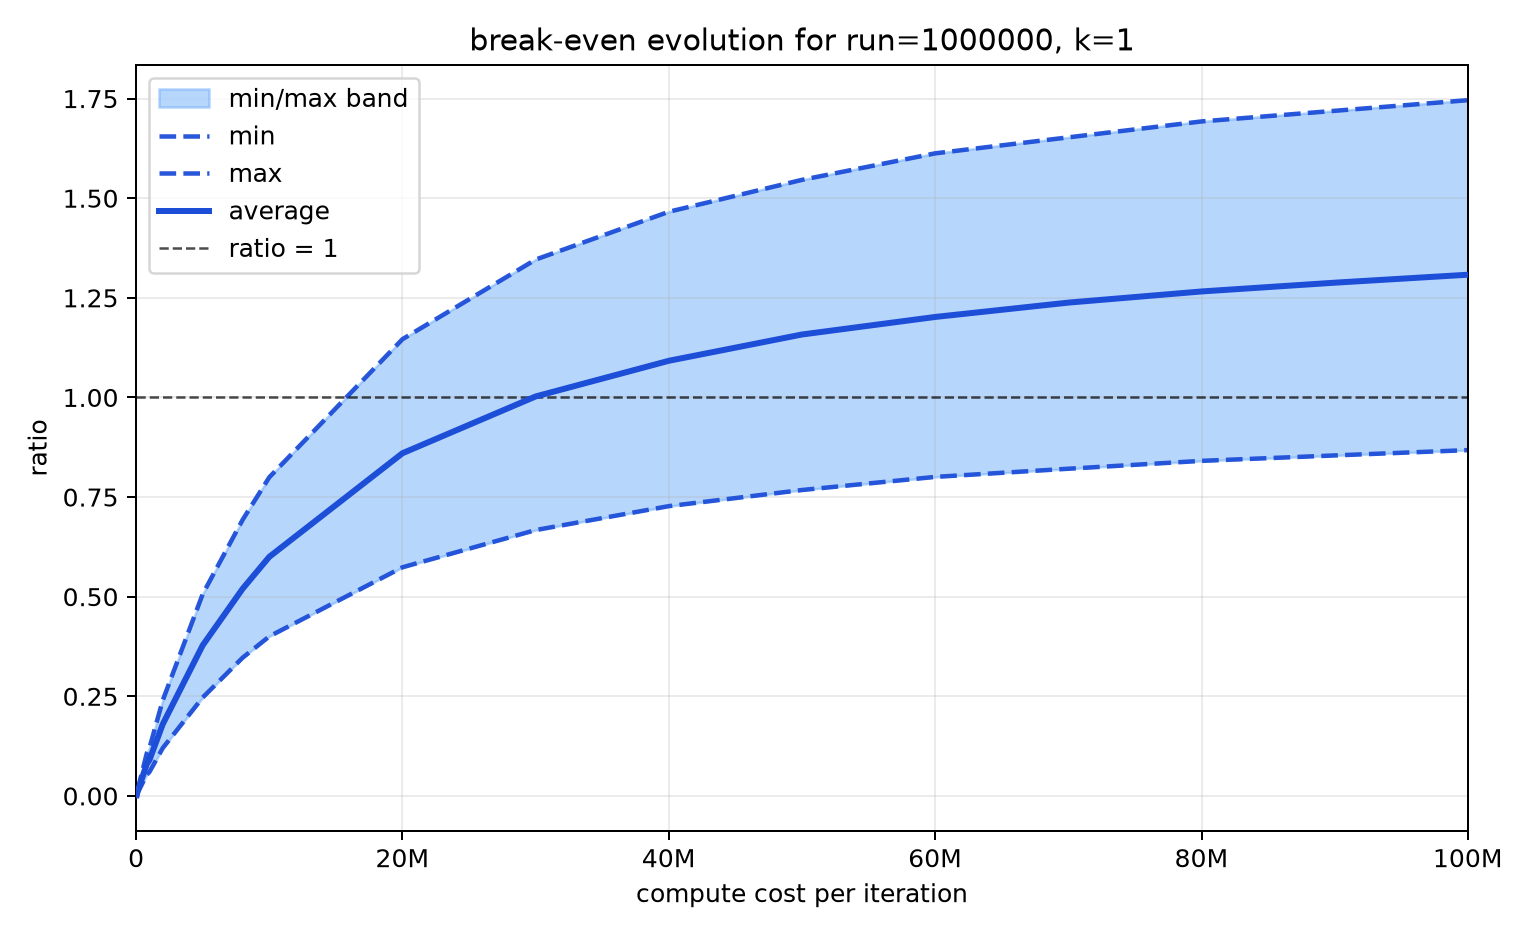
\includegraphics[width=0.8\linewidth]{img/plots/15m_break_even_focus_run_1000000_k_1.png}
    \caption{Threshold for 1 error over a 1.000.000 runs enclave assuming a 15M cost for load and save}
    \label{fig:15m_threshold_k}
\end{figure}

\begin{figure}[H]
    \centering
    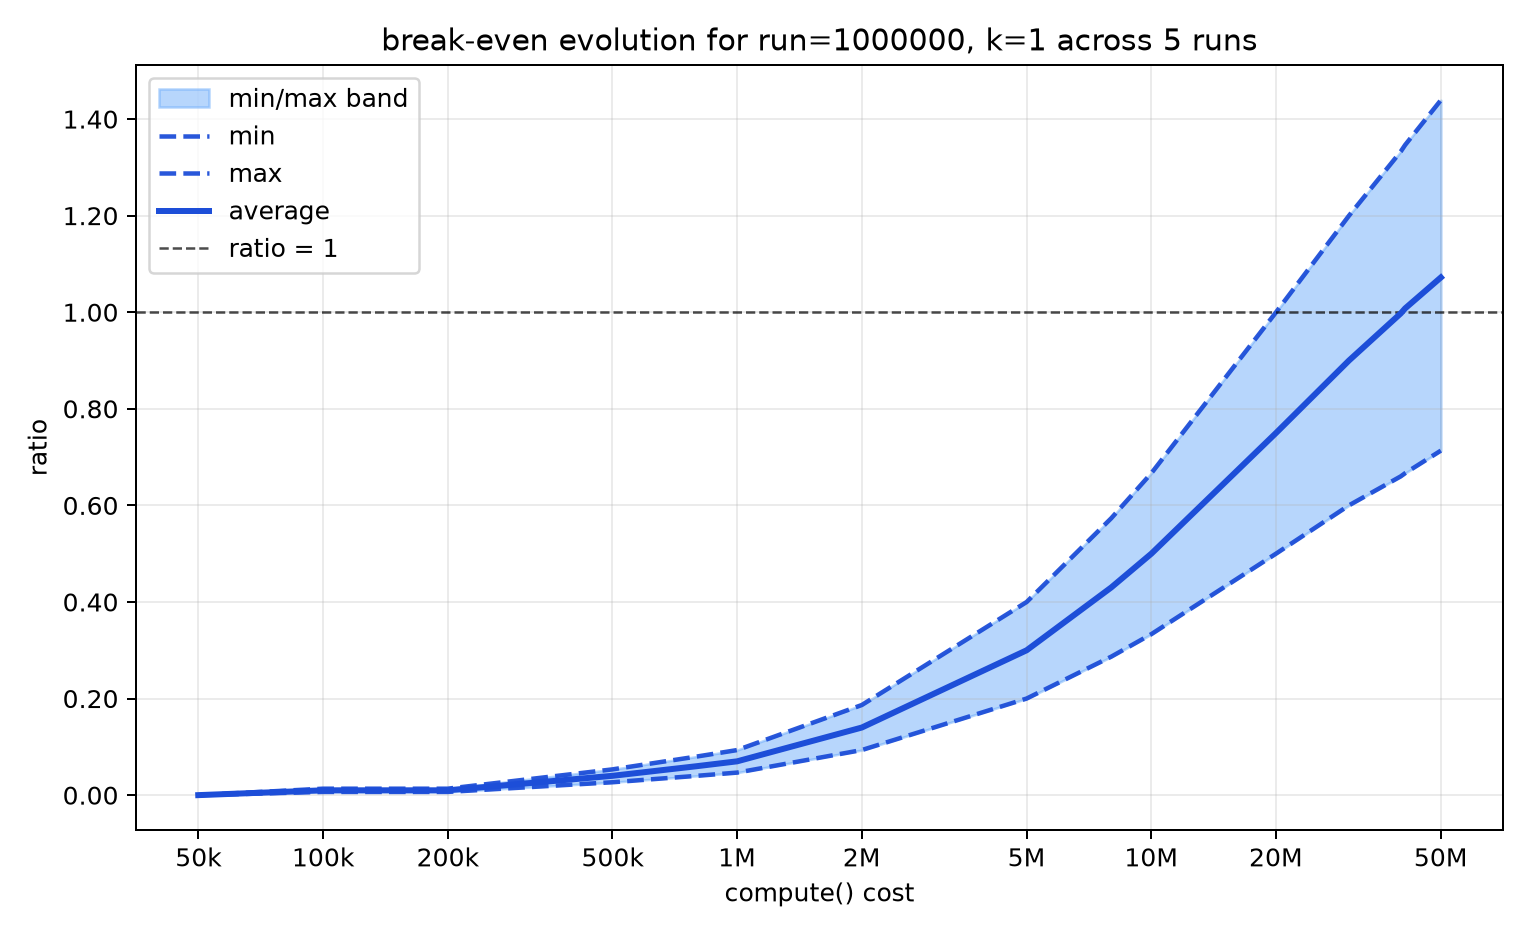
\includegraphics[width=0.8\linewidth]{img/plots/20m_break_even_focus_run_1000000_k_1.png}
    \caption{Threshold for 1 error over a 1.000.000 runs enclave assuming a 20M cost for load and save}
    \label{fig:20m_threshold_k}
\end{figure}

\begin{figure}[H]
    \centering
    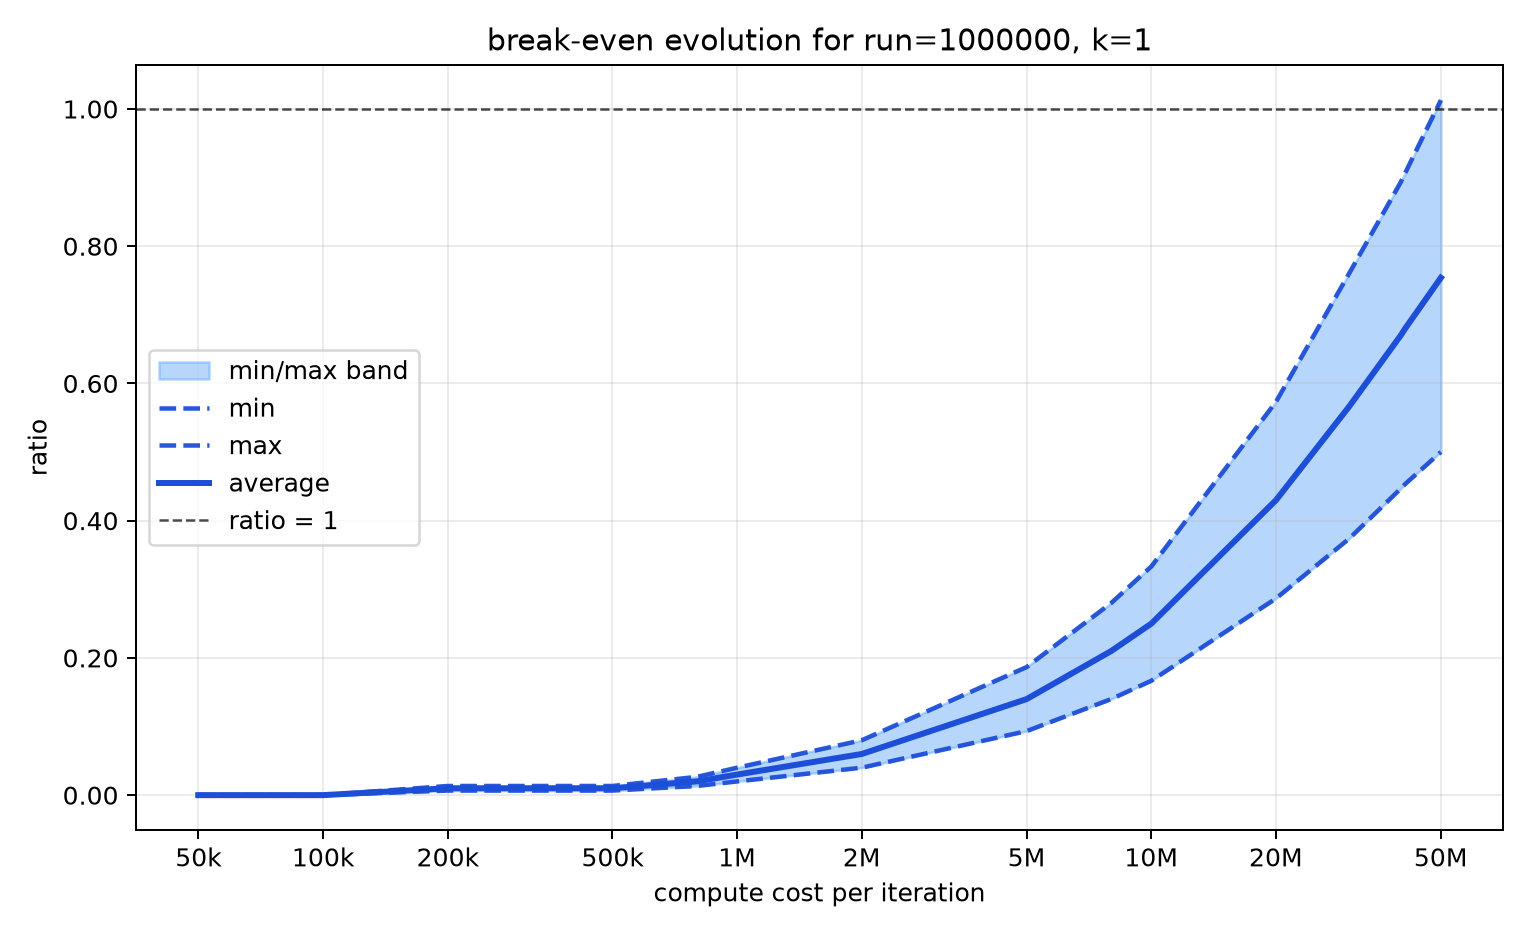
\includegraphics[width=0.8\linewidth]{img/plots/50m_break_even_focus_run_1000000_k_1.png}
    \caption{Threshold for 1 error over a 1.000.000 runs enclave assuming a 50M cost for load and save}
    \label{fig:50m_threshold_k}
\end{figure}


\subsubsection{K = $[0-9]$}
Next we show the result, without the maximal and minimal bounds for the first $9$ errors.
These ones highlight the plateau effect even when working with possibly more faults.
As we explained above, the plateau appears because as we increase $C_{compute}$ to balance the other ones, the two sides equals out and both $C_{save}$ and $C_{load}$ become insignificant.
Our intuition can also help us understand that effect as both $C_{checkpoint}$ and $C_{no_checkpoint}$ both use $C_{compute}$
Nevertheless, as $K$ grows, the first slope gets steeper, resulting in a \textbf{logarithmic function}. 
We can explain that with the effective cost of the save being shrinked by more faults, in both intuition and equation \ref{eq:threshold_ratio}.
The the balance between the two effect gives some kind of saturation slop.

\begin{figure}[H]
    \centering
    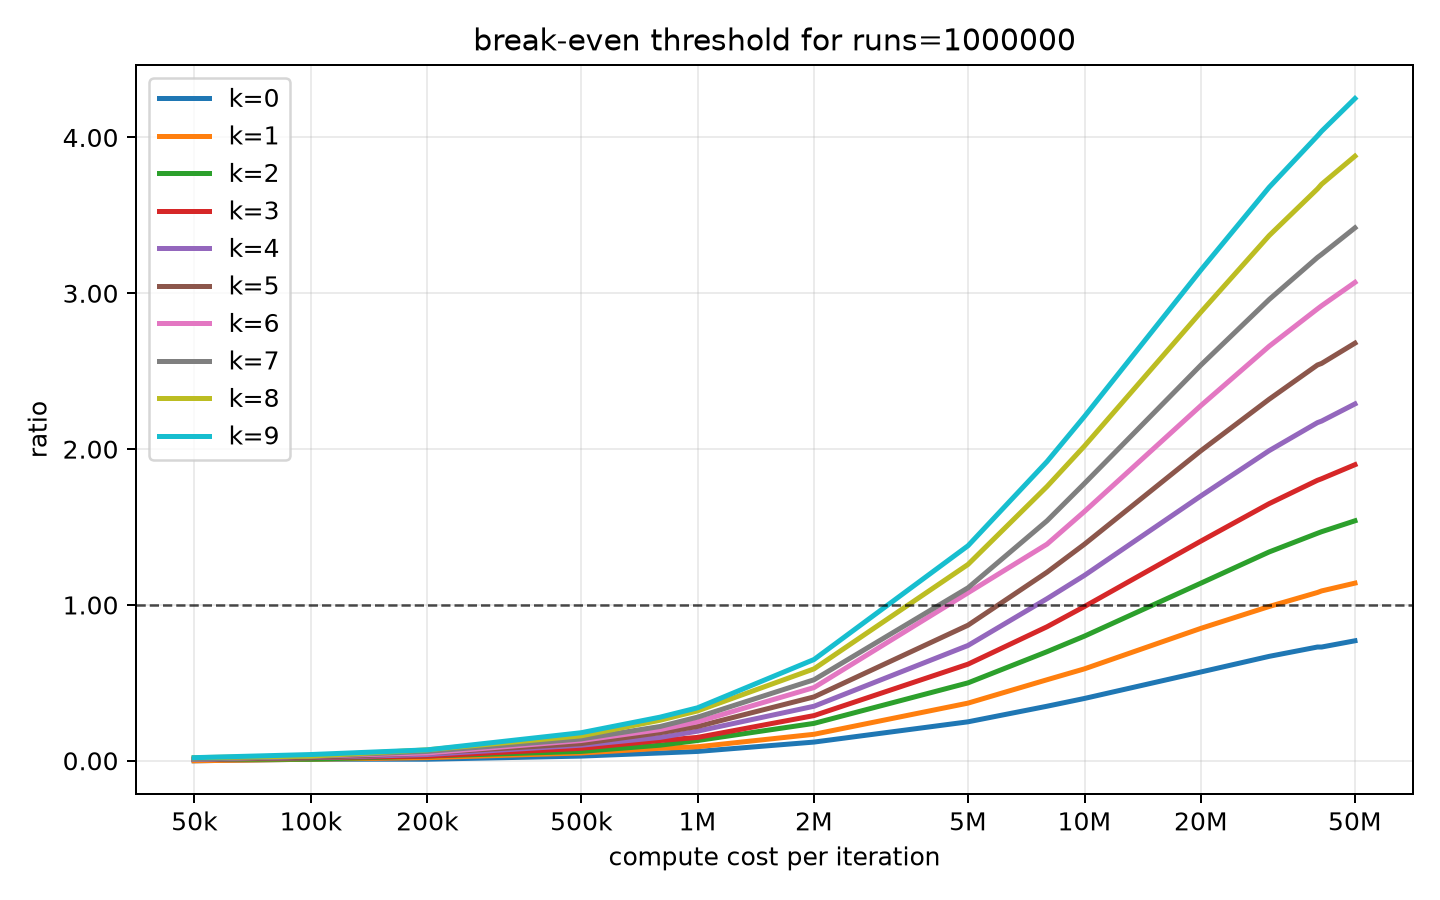
\includegraphics[width=0.8\linewidth]{img/plots/15m_break_even_thresholds_runs_1000000.png}
    \caption{Threshold ratio for k=$[0-9]$, over a 1.000.000 runs enclave assuming a 15M cost for load and save}
    \label{fig:15m_threshold_all_k}
\end{figure}

\begin{figure}[H]
    \centering
    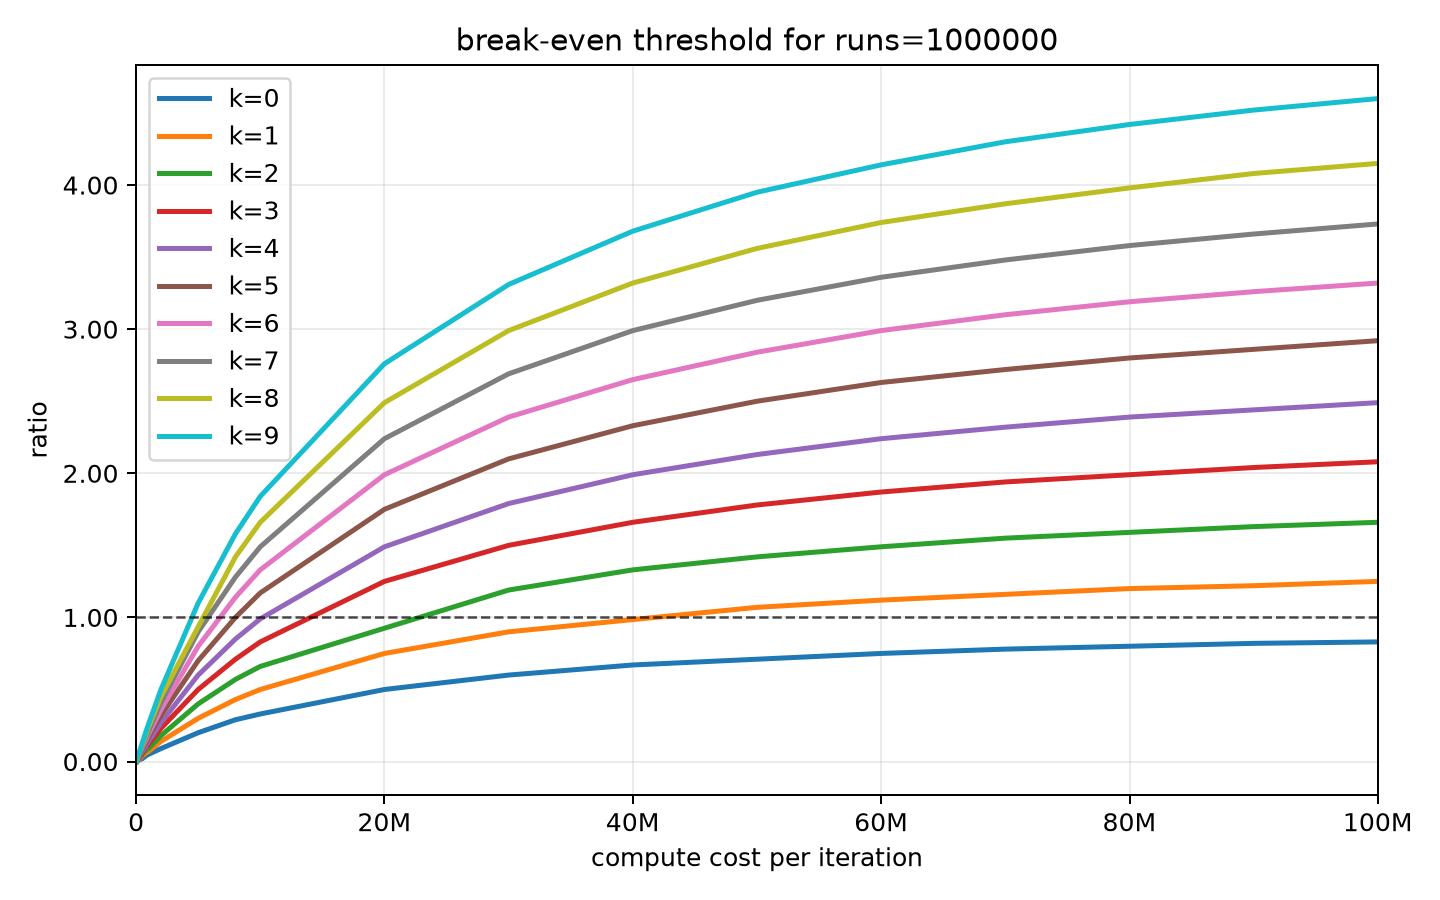
\includegraphics[width=0.8\linewidth]{img/plots/20m_break_even_thresholds_runs_1000000.png}
    \caption{Threshold ratio for k=$[0-9]$, over a 1.000.000 runs enclave assuming a 20M cost for load and save}
    \label{fig:20m_threshold_all_k}
\end{figure}

\begin{figure}[H]
    \centering
    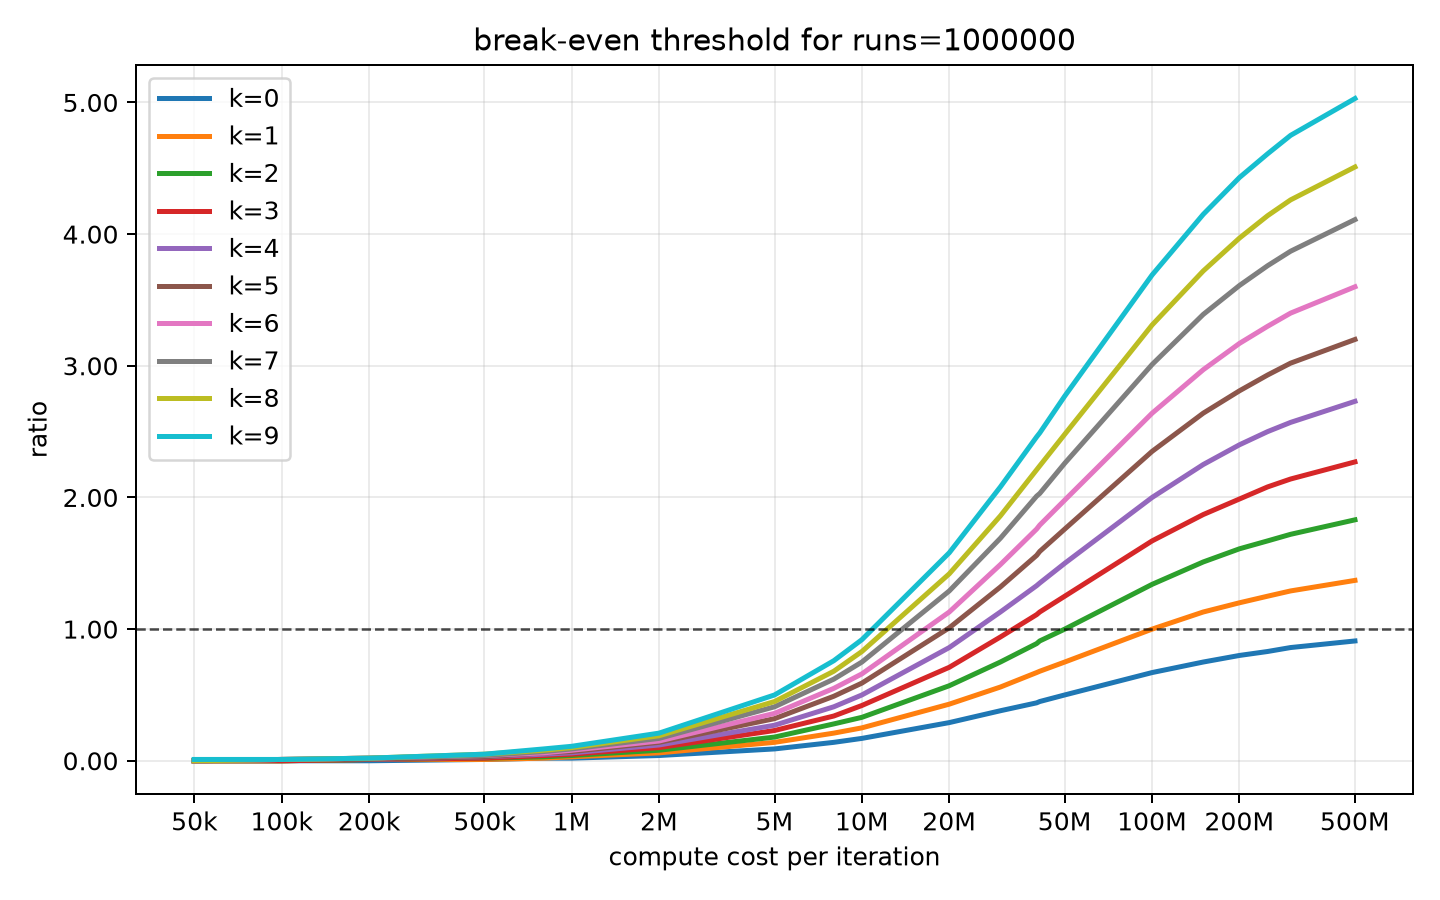
\includegraphics[width=0.8\linewidth]{img/plots/50m_break_even_thresholds_runs_1000000.png}
    \caption{Threshold ratio for k=$[0-9]$, over a 1.000.000 runs enclave assuming a 50M cost for load and save}
    \label{fig:50m_threshold_all_k}
\end{figure}

\subsubsection{Checkpoint interval}
We can see that making a save every $2$ steps already yields much greater results as they cut the cost needed for the threshold by $2$.
In our implementation, we will see better results until $X\leq 13$, after that, the recovery cost starts balancing out the gains made by avoiding the save computation.
\begin{figure}[H]
    \centering
    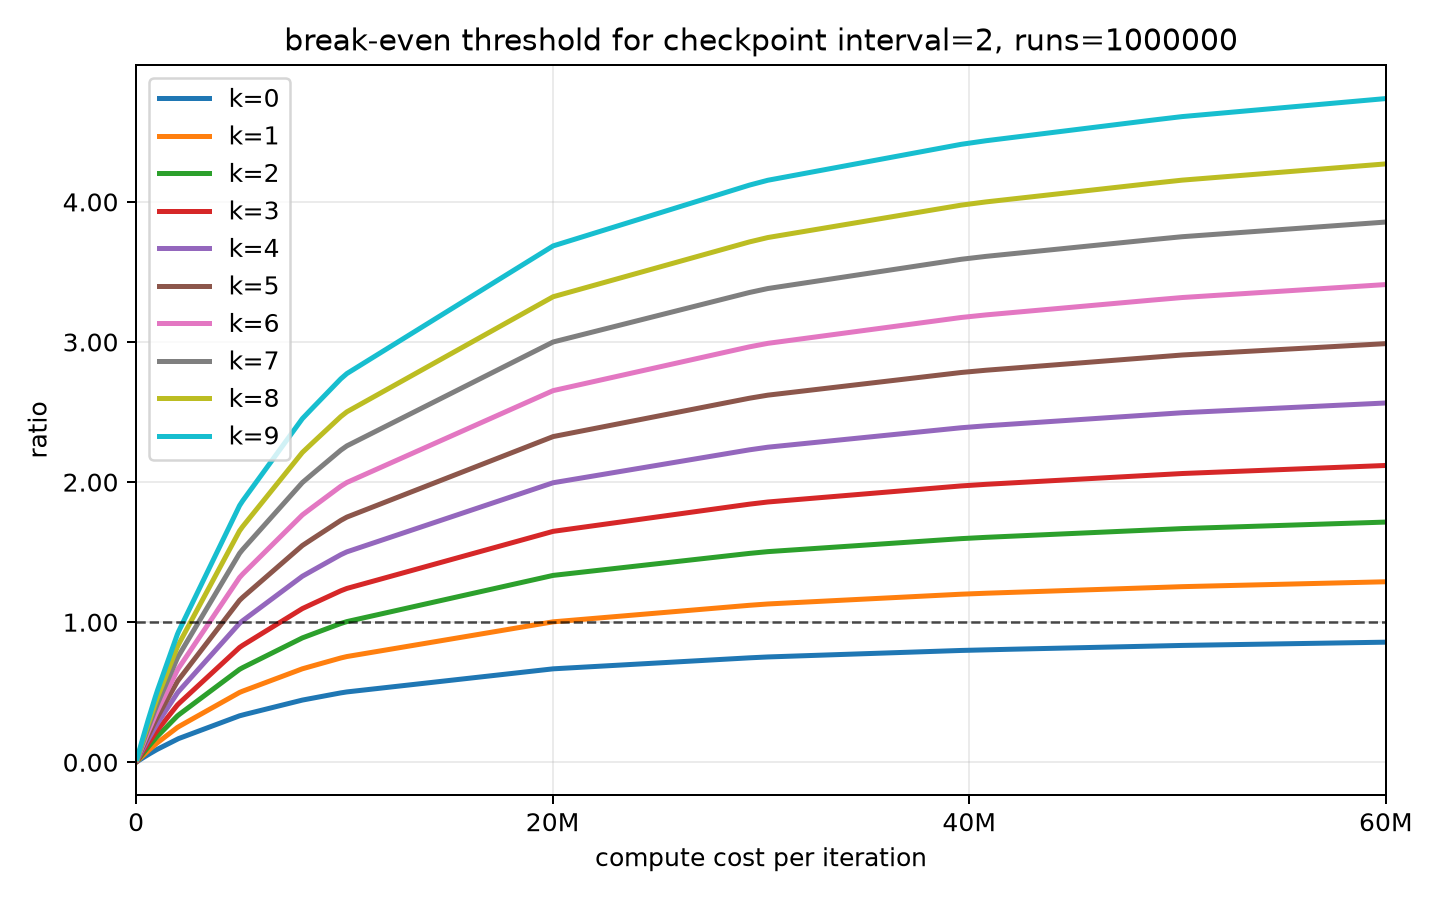
\includegraphics[width=0.8\linewidth]{img/plots/20m_checkpoint_interval_2_run_1000000.png}
    \caption{Checkpoint interval = $2$ threshold ratio for k=$[0-9]$, over a 1.000.000 runs enclave assuming a 20M cost for load and save}
    \label{fig:20m_checkpoint_interval}
\end{figure}


\subsection{Cycle cost per operation}
\label{sub:cycle_cost}
This part is a recap of each possible main operation of the enclave during an iteration.
The values below are averaged over $1000$ runs, they inclued the material derivation as \textit{cached} from the sealing and unsealing and the data being sealed can be found in the Section \ref{subsub:data-struct}.
We used the \verb|EAPP_CYCLE_BREAKDOWN_TESTING| macro to render these tables.
\\

However, even using a smoothing method to avoid outliers, QEMU is not as reliable as FireSim \cite{keystone-web} in terms of cycle usage.
Having this in mind, we could not run FireSim because of the long setup it needs.
In fact, it has a whole documentation over at : \href{https://chipyard.readthedocs.io/en/latest/simulation/fpga-accelerated-simulation/#firesim-sim-intro}{Chipyart documentation}.
In order to use it, we would need to :
\begin{itemize}
    \item setup a FireSim Manager instance on Amazon EC2
    \item deploy it to Amazon AWS FPGAs using FireSim
    \item install the Chipyard repo onto it
    \item use it as an external library in Chipyard
\end{itemize}
The following results must then be interpreted while keeping this limitation in mind.

\begin{table}[H]
    \centering
    \label{tab:seal_cycle_breakdown}
    \begin{tabular}{|l|r|}
        \hline
        Component & Cycles \\
        \hline
        Key derivation & 21,873 \\
        Seal preparation & 9,366 \\
        AES-CTR encryption & 9,698,615 \\
        CBC-MAC tag & 9,939,972 \\
        Blob copy out & 16,089 \\
        Total seal cost & 19,664,042 \\
        \hline
    \end{tabular}
    \caption{Seal cycle cost breakdown}

\end{table}

\begin{table}[H]
    \centering
    \label{tab:unseal_cycle_breakdown}
    \begin{tabular}{|l|r|}
        \hline
        Component & Cycles \\
        \hline
        Blob copy in & 8,367 \\
        CBC-MAC tag recomputation & 9,992,689 \\
        Tag compare & 1,697 \\
        AES-CTR decryption & 9,702,006 \\
        Blob copy out & 13,409 \\
        Total unseal cost & 19,718,168 \\
        \hline
    \end{tabular}
    \caption{Unseal cycle cost breakdown}

\end{table}

\begin{table}[H]
    \centering
    \label{tab:cpmpute_cycle_costs}
    \begin{tabular}{|l|r|}
        \hline
        Operation & Cycles \\
        \hline
        Computation & 275,100 \\
        \hline
    \end{tabular}
    \caption{compute costs}
\end{table}

\subsection{Data cost}
\label{sub:data-cost}

The benchmarked plaintext checkpoint has size $8208$ bytes, and the measured costs are $19.664.042$ cycles for sealing and $19.718.168$ cycles for unsealing. 
Using the plaintext size as denominator gives the per-byte averages:
\begin{align}
    C_{\text{1\_byte\_seal}} &\approx \lceil\frac{19.664.042}{8208}\rceil \approx 2396 \\
    C_{\text{1\_byte\_unseal}} &\approx \lceil\frac{19.718.168}{8208}\rceil \approx 2402 \\
    C_{\text{1\_byte\_roundtrip}} &\approx 4798
\end{align}

\subsection*{Time cost}
As for the \textit{data cost}, the time can be derived from the cycle cost.
as 

\section{Cybersecurity}
Now that the computation and data analysis is done, we will address the cybersecurity assumptions and requirements.

\subsection{Security objectives}
As stated in \ref{sec:threat-model}, there are four security objectives that will be looked upon.
We will discuss of why they hold and what are the limitations.
The claims can be checked using the corresponding macros in (Section \ref{chap:experimental_setup}).

%\item \textbf{Confidentiality}: checkpoint contents unreadable to host
%\item \textbf{Integrity/authenticity}: tampered blob is detected, rejected and leaks no information (response time analysis) 
%\item \textbf{Atomicity}: no undefined state from interrupted checkpoint writes
%\item \textbf{Unclonability}: can't clone device from checkpoint data alone
\subsubsection{Confidentiality}
Confidentiality means that the checkpoint is, at any time, opaque from the host. 
An attacker can, indeed, not read the saved checkpoint because of the \verb|aes_encrypt_ctr()| function provided by Keystone.   
In our implementation, the rewind state to save is read from the stack, placed into a plain text checkpoint storage and then sealed using the encryption key derived from Keystone data sealing key (Section \verb|get_sealing_key()| \ref{sec:data-sealing}) and the iv (the checkpoint sequence).
After that, a tag is done over the ciphertext using the authentification key to block anyone from tampering without notice.
The resulting sealed checkpoint blob is then sent to the host along with the iv and the tag.


\subsubsection{Integrity}
We now have to consider the possible tampering and side-attacks, the former is that that the attackers tries to mess with the blob bytes directly, which is not plausible under the scheme \textit{over a fixed length message}. 
Another attack is to obtain side informations to deduce information. This can be time to compute the tag or reloading the enclave by destroying it at every save edge call and XORing the resulting initial ciphertexts.
The first one is addressed using a simple, constant time comparison function that always passes over the whole sequence instead of a memcmp() that stops as soon a one byte is wrong.
using memcmp(), or any non constant time comparison function would lead to a time of authentification leak in our scenario.
The second one is, in our case, directly addressed by the inherent deterministic mechanism of the enclave, the initial state, will always be the same as the one being compiled (whatever a and b are).
Moreover, the checkpoint sequence also follows this rule. Making a XOR of a possibly same ciphertext with different IVs simply not possible. 

\subsubsection{Atomicity}
Atomicity states that we cannot have an undefind saved state. Based on the two last objectives, a maliciously modified state is not something to scared of.
However, could an attacker stops the enclave at the perfect time in order to create a chimera state.
The answer is no. In fact, the only real abilities, to this regard, of the attacker is to cut the power of the enclave. 
The only outcome of this scenario is to also stop the host and the SM, effectively stopping the whole system.
The protection of a whole system is not in the scope of this thesis.
Nevertheless, the state, checkpoint of this state and sealed checkpoint are being kept separated for this purpose. 
Whenever one changes, it doesn't always affect the others.

Another idea would be to compromise the PMP hardware itself, this scenario is not in the scope of this thesis as it is assumed to be sound in runtime to malicious programs.
Even only destroying the entry would result in a call to the SM, and a move of the enclave from this hardware space.

\subsubsection{Unclonability}
We consider a device to be cloned if we can replicate the exact behaviour given a sealed state.
This is only possible for a program that has the \textbf{exact} same hash as the EAPP and is ruled by the SM.
Otherwise, the keys won't correspond and the attacker will not be able to read or to use the sealed data.
In addition to that, there is no point in time where the plaintext is exposed.
We can thus safely rely on Keystone data sealing to make the sealed checkpoint unusable for someone that is not the enclave EAPP.


%%%%%%%%%%%%%%%%%%%%%%%% Discussion & Future work %%%%%%%%%%%%%%%%%%%%%%%%
\chapter{Discussion and Future work}
\label{chap:discussion}

\section{Discussion}
The results show that rewind is not a universal replacement for a normal execution path, but it becomes attractive as soon as the enclave performs enough useful work between faults to amortize the cost of saving and restoring state. 
In practice, the relevant question is not whether checkpointing is expensive in absolute terms, but whether the saved execution time is larger than the overhead introduced by sealing, loading, and recovery. 
That is why the break-even threshold and the checkpoint interval are the two most important quantities in this thesis.
Moreover, a fault could cause a long time shutdown in practice for long running jobs.
Recovering from that, even in a non optimal setup, could be useful in time concerns.
\\

The threshold analysis confirms that the cost of checkpointing is dominated by the fixed overhead of saving the enclave state.
When the compute cost is small, the mechanism is difficult to justify because the enclave spends most of its time protecting work rather than doing work.
As the compute cost increases, the same overhead becomes easier to absorb, and rewind starts to make sense for longer-running or more repetitive tasks.
This means the mechanism is most useful for workloads that run long enough to tolerate occasional recovery cost, such as batch-style processing, repeated iterations, or tasks that may have to survive a long interruption.
 \\

The checkpoint interval analysis refines that conclusion.
Saving too often reduces the amount of work lost after a fault, but it also increases the number of expensive seal operations.
Saving too rarely lowers checkpoint overhead, but it increases the amount of recomputation after a failure.
The optimal interval therefore depends on the relative cost of computation, checkpointing, and fault recovery, and on the expected number of faults over the lifetime of the enclave.
In other words, rewind is only practical if the application can choose an interval that matches its own cost profile rather than relying on a fixed policy for every workload.
Another point about the the saving ratio is for mixed critical systems. The period could be mapped to a criticality level so that most important task get reloaded quicker while the others could still recover.
Thus, all benefiting from the gains of rewinding while mitigating its costs.
\\

From a security point of view, the model is useful because it contains the threat outside the enclave while keeping the recovery state protected. The host remains unreliable, but the checkpointed state can still be restored safely as long as the sealing and integrity assumptions hold.
This gives a clear separation of responsibilities: the untrusted world can fail, delay, or discard the enclave, but it should not be able to read or modify the protected checkpoint without detection. 
The mechanism is therefore acceptable as a resilience layer only if the enclave boundary, the sealing key, and the state-restore path remain trustworthy.
\\

The crypto cost also matters in the discussion. The current sealing approach is correct for the implementation, but it contributes directly to the runtime overhead and therefore to the break-even point. 
Any lighter checkpoint protection scheme would improve the usefulness of rewind by lowering the fixed cost of each save and making shorter checkpoint intervals more affordable. 
This is why the cryptographic choice is not just a security detail: it is part of the performance model.
\\

Overall, the thesis supports a conditional answer. 
Rewind is useful when the enclave does enough work between faults, when the checkpoint interval is chosen carefully, and when the security boundary can be trusted even though the host cannot. 
It is less convincing for tiny workloads, for very rare faults, or for applications that cannot afford the extra checkpoint cost. 
That makes the mechanism promising, but only in the class of long-running protected tasks where recovery cost is smaller than the work it saves.


\section{Future Work}

The following directions extend the current rewind design without changing its basic goal.
They focus on making the checkpoint policy more adaptable, the protection layer lighter, and the recovery path more realistic.

\subsection{Mixed criticality}
The current implementation treats every enclave run as if it had the same level of urgency and the same recovery policy. 
A natural follow-up would be to support mixed-criticality workloads, where the enclave can distinguish between essential work that must always be preserved and optional work that can be recomputed or discarded more aggressively.

This would make the checkpoint policy more flexible. A high-criticality task could save state more often and use a stricter recovery path, while a lower-criticality task could accept larger intervals or even cheaper checkpoint protection. 
In that setting, the checkpoint interval would no longer be a single global parameter, but a policy that depends on the value of the task being protected.

Such a design would also make the discussion on usefulness more realistic. 
Real applications rarely consist of one homogeneous loop, and a mixed-criticality model would let the rewind mechanism adapt to different phases of the same application instead of forcing one compromise for the whole execution.

Nevertheless, the results on checkpoint intervals could be used to implement a higher level critical model, that operates at the enclave level.
Making each enclave at a given level and then mapping this to a period, the highest priority getting the lowest period. 
Note that that would need some fine tuning and system design in order to fit the hardware capabilites and task deadlines.

\subsection{Modern lightweight cryptoscheme}
The current sealing layer has been chosen because of its supposed soundness (relying on Keystone data sealing), but it is not necessarily the best choice if the goal is to minimize recovery overhead. 
A useful future direction would be to replace it with a more lightweight cryptographic construction that still provides confidentiality and integrity while reducing the cost of every save and load operation.

This matters because the cryptographic cost appears directly in the checkpointing model. Any reduction in sealing overhead would lower the break-even threshold and make shorter checkpoint intervals less expensive. 
It would also improve the practicality of rewind for workloads with smaller compute cost, which are currently the least favorable case for the mechanism.

Another possible improvement would be to separate the cryptographic policy from the checkpoint logic more clearly using hardware enforced cryptography for example or built-in more specialised schemes. 
That would make it easier to compare several schemes under the same benchmark framework and to measure whether the gain is mostly coming from a better algorithm, a smaller state, or a better implementation choice.

\subsection{More complex fault model}
\label{sub:fault-model}
The thesis currently assumes a relatively simple fault model, which is enough to show the basic behavior of rewind but not enough to describe every realistic failure pattern. 
A stronger follow-up would be to study burst faults, correlated faults, and repeated faults on the same execution window, since those cases can change the usefulness of checkpointing quite dramatically.

This would also let the model capture the difference between isolated failures and adversarial or unstable environments. 
If the faults are no longer independent, then the expected recomputation cost changes, the optimal checkpoint interval changes, and the threshold analysis becomes more difficult but also more representative of real deployments.

From an implementation point of view, a richer fault model would also allow the enclave to react differently depending on the failure history. 
For example, the system could decide to shorten the checkpoint interval after repeated faults or to switch to a degraded recovery mode when the fault rate becomes too high.

\subsection{Enclave Complexity on backup}
\label{sub:back-complexity}
The current backup path is intentionally simple: it restores the enclave state and resumes execution without introducing a richer failure-management policy. 
A further step would be to study how the complexity of the backup enclave affects both security and performance.

This is important because the backup path is part of the trusted computing base. 
The more logic it contains, the more careful one must be about correctness, memory usage, and attack surface. 
At the same time, a more capable backup could support better policy decisions, richer diagnostics, or more fine-grained restoration rules.

It would also be useful to measure how much extra checkpoint metadata is needed as the backup logic grows. 
If recovery requires more state, then the cost of saving and validating that state may erase part of the benefit of rewind. 
Studying that tradeoff would clarify how far the design can scale (up or down) before the backup mechanism becomes too complex to remain attractive.



%%%%%%%%%%%%%%%%%%%%%%%% Conclusion %%%%%%%%%%%%%%%%%%%%%%%%
\chapter{Conclusion}
\TODO{conclusion}


\printbibliography
%\bibliographystyle{unsrt}
%\bibliography{ref}
\newpage

\appendix
\chapter*{Appendix}
\label{chap:appendix}
\section*{Rewind source code}
\label{file:source-code}
These files (and their usage) can be found in the repository: \github and they are compiled (downloadable) in this pdf.

\begin{verbatim}
# scripts
make-examples.sh
make-run.sh
run-rewind.sh

# source files
examples/rewind/
  CMakeLists.txt
  eapp/
    checkpoint.c
    checkpoint.h
    common.c
    common.h
    crypto.c
    crypto.h
    eapp_test.c
    eapp_test.h
    fault.c
    fault.h
    rewind.c    # enclave file
  host/
    host_test.cpp
    host_test.hpp
    host.cpp
    host.hpp
\end{verbatim}

\subsection*{\texttt{eapp/checkpoint}}
\label{file:checkpoint}
\srcattach{src/rewind/eapp/checkpoint.c}{examples/rewind/eapp/checkpoint.c}
\srcattach{src/rewind/eapp/checkpoint.h}{examples/rewind/eapp/checkpoint.h}

\subsection*{\texttt{eapp/eapp\_test}}
\label{file:eapp_test}
\srcattach{src/rewind/eapp/eapp_test.c}{examples/rewind/eapp/eapp\_test.c}
\srcattach{src/rewind/eapp/eapp_test.h}{examples/rewind/eapp/eapp\_test.h}

\subsection*{\texttt{eapp/crypto}}
\label{file:crypto}
\srcattach{src/rewind/eapp/crypto.c}{examples/rewind/eapp/crypto.c}
\srcattach{src/rewind/eapp/crypto.h}{examples/rewind/eapp/crypto.h}

\subsection*{\texttt{eapp/common}}
\label{file:common}
\srcattach{src/rewind/eapp/common.c}{examples/rewind/eapp/common.c}
\srcattach{src/rewind/eapp/common.h}{examples/rewind/eapp/common.h}

\subsection*{\texttt{eapp/fault}}
\label{file:fault}
\srcattach{src/rewind/eapp/fault.c}{examples/rewind/eapp/fault.c}
\srcattach{src/rewind/eapp/fault.h}{examples/rewind/eapp/fault.h}

\subsection*{\texttt{eapp/rewind.c}}
\label{file:rewind}
\srcattach{src/rewind/eapp/rewind.c}{examples/rewind/eapp/rewind.c}

\subsection*{\texttt{host/host\_test}}
\label{file:host}
\srcattach{src/rewind/host/host_test.cpp}{examples/rewind/host/host\_test.cpp}
\srcattach{src/rewind/host/host_test.hpp}{examples/rewind/host/host\_test.hpp}

\subsection*{\texttt{host/host}}
\label{file:host_test}
\srcattach{src/rewind/host/host.cpp}{examples/rewind/host/host.cpp}
\srcattach{src/rewind/host/host.hpp}{examples/rewind/host/host.hpp}

\subsection*{\texttt{CMakeLists.txt}}
\label{file:CMake}
\srcattach{src/rewind/CMakeLists.txt}{examples/rewind/CMakeLists.txt}

\section*{Scripts}
\label{file:scripts}

\subsection*{\texttt{make-examples.sh}}
\label{file:make-examples}
\srcattach{src/make-examples.sh}{./make-examples.sh}

\subsection*{\texttt{run-rewind.exp}}
\label{file:run-rewind}
\srcattach{src/run-rewind.exp}{./run-rewind.exp}

\subsection*{\texttt{make-run.sh}}
\label{file:make-run}
\srcattach{src/make-run.sh}{./make-run.sh}

\section*{README}
\label{file:readme}
\srcattach{src/README.md}{README.md}



\end{document}